\documentclass[11pt]{aghdpl}

\usepackage[english,polish]{babel}
\usepackage{polski} % Użyj polskiego łamania wyrazów (zamiast domyślnego angielskiego).
\usepackage[utf8]{inputenc}

% dodatkowe pakiety
\usepackage{afterpage}
\usepackage{mathtools}
\usepackage{amsfonts}
\usepackage{amsmath}
\usepackage{amsthm}
\usepackage{float} 
\usepackage{realboxes}
\usepackage{xpatch}
\usepackage{lscape} % landscape
\usepackage{pdfpages} % Do dodawnaie stron pdf jako część dokumentu (nie lstlisting)
\usepackage{emptypage} % Paczka wyłącza pokazywanie numeru strony oraz nagłówków na pustych stronach
\usepackage{siunitx}

% Dzięki temu będzie się dało kopiować tekst który ma polskie literki
% see: https://tex.stackexchange.com/questions/57915/cannot-copy-letters-with-diacritics-from-pdflatex-pdf
\usepackage{lmodern}
\usepackage{listings}
\usepackage{multicol}

% Polskie literki w listingach:
\lstset{
    literate=
    {ą}{{\k{a}}}1 {Ą}{{\k{A}}}1 
    {ł}{{\l{}}}1 {Ł}{{\L{}}}1 
    {ń}{{\'n}}1 {Ń}{{\'N}}1 
    {ę}{{\k{e}}}1 {Ę}{{\k{E}}}1 
    {ś}{{\'s}}1 {Ś}{{\'S}}1 
    {ż}{{\.z}}1 {Ż}{{\.Z}}1 
    {ó}{{\'o}}1 {Ó}{{\'O}}1 
    {ź}{{\'z}}1 {Ź}{{\'Z}}1 
    {ć}{{\'c}}1 {Ć}{{\'C}}1
}


% Definicja listingu dla Dockerfile
% https://gordonlesti.com/custom-code-highlighting-in-latex/
\lstdefinelanguage{Dockerfile}
{
  morekeywords={FROM, RUN, CMD, LABEL, MAINTAINER, EXPOSE, ENV, ADD, COPY,
    ENTRYPOINT, VOLUME, USER, WORKDIR, ARG, ONBUILD, STOPSIGNAL, HEALTHCHECK,
    SHELL},
  morecomment=[l]{\#},
  morestring=[b]"
}

% Definicja listingu dla CMAKE
\lstdefinelanguage{cmake}
{
  morekeywords={set, cmake_minimum_required, project, add_executable, target_include_directories, include, target_link_libraries, file, add_library, set_target_properties, if, endif, list, foreach, endforeach, add_subdirectory, get_directory_property, get_filename_component, function, endfunction, execute_process, ExternalProject_Add, target_link_directories, message, else},
  morecomment=[l]{\#},
  morestring=[b]"
}

\lstdefinelanguage{Cmd}
{
    moredelim=[s][\color{red}\bfseries]{user@host}{\$},
    morekeywords={}
}

\definecolor{darkgreenforcomments}{rgb}{0.0,0.26,0.15}

\lstdefinelanguage{yaml}
{
  keywords={true,false,null,y,n},
  sensitive=false,
  comment=[l]{\#},
  morecomment=[s]{/*}{*/},
  commentstyle=\color{darkgreenforcomments}\ttfamily,
  stringstyle={\color{blue}\mdseries},
  moredelim=[l][\color{orange}]{\&},
  moredelim=[l][\color{magenta}]{*},
  moredelim=**[il][\color{red}{:}\color{blue}]{:},
  morestring=[b]',
  morestring=[b]"
}

\definecolor{lgray}{gray}{0.96}
\definecolor{lbcolor}{rgb}{0.9,0.9,0.9}
\lstset{
    framesep=2pt,
    basicstyle=\ttfamily,
    breaklines=true,
    breakatwhitespace=true,
    basicstyle=\footnotesize,
    aboveskip={0.75\baselineskip},
    columns=fixed,
    showstringspaces=false,
    breaklines=true,
    prebreak = \raisebox{0ex}[0ex][0ex]{\ensuremath{\hookleftarrow}},
    frame=single,
    rulecolor=\color{lgray},
    showtabs=false,
    showspaces=false,
    showstringspaces=false,
    backgroundcolor=\color{lgray},
    identifierstyle=\ttfamily,
    keywordstyle=\color[rgb]{0,0,1},
    commentstyle=\color[rgb]{0.0,0.26,0.15},
    stringstyle=\color[rgb]{0.627,0.126,0.941}
}

% Padding w podpisach do listingow i obrazkow
% ustawiony na 0
\captionsetup[lstlisting]{ margin=0pt}
\captionsetup[figure]{ margin=0pt}
\captionsetup[table]{ margin=0pt}



\makeatletter
\xpretocmd\lstinline{\Colorbox{lgray}\bgroup\appto\lst@DeInit{\egroup}}{}{}
\makeatother

\usepackage[hidelinks]{hyperref}

% --- < bibliografia > ---
%
% TODO: Dla TeXstudio warto przeczytać poniższe!
% UWAGA: Żeby bibliografia działała gdy używamy TeXstudio, to należy zmodyfikować quick build w opcjach, tak aby wykonywane były polecenia:
% 	PdfLaTeX
% 	BibTeX
% 	PdfLaTeX
% 	PdfLaTeX
%
% Więcej informacji na:
% 	https://tex.stackexchange.com/a/216325
%

\usepackage[
	backend=bibtex,
	style=numeric,
	sorting=none,
	% Zastosuj styl wpisu bibliograficznego właściwy językowi publikacji.
	language=autobib,
	autolang=other,
	% Zapisuj datę dostępu do strony WWW w formacie RRRR-MM-DD.
	urldate=iso8601,
	% Nie dodawaj numerów stron, na których występuje cytowanie.
	backref=false,
	% Podawaj ISBN.
	isbn=true,
	% Nie podawaj URL-i, o ile nie jest to konieczne.
	url=false,
	% Ustawienia związane z polskimi normami dla bibliografii.
	maxnames=50,
]{biblatex}

\usepackage{csquotes}
% Ponieważ `csquotes` nie posiada polskiego stylu, można skorzystać z mocno zbliżonego stylu chorwackiego.
\DeclareQuoteAlias{croatian}{polish}

% Bibliografia musi być uzupełniona w tym pliku:
\addbibresource{bibliografia.bib}

% Nie wyświetlaj wybranych pól.
%\AtEveryBibitem{\clearfield{note}}


% ------------------------
% --- < listingi > ---

% Użyj czcionki kroju Courier.
\usepackage{courier}

\lstloadlanguages{TeX}

% Polskie literki:
\lstset{
	literate={ą}{{\k{a}}}1
           {ć}{{\'c}}1
           {ę}{{\k{e}}}1
           {ó}{{\'o}}1
           {ń}{{\'n}}1
           {ł}{{\l{}}}1
           {ś}{{\'s}}1
           {ź}{{\'z}}1
           {ż}{{\.z}}1
           {Ą}{{\k{A}}}1
           {Ć}{{\'C}}1
           {Ę}{{\k{E}}}1
           {Ó}{{\'O}}1
           {Ń}{{\'N}}1
           {Ł}{{\L{}}}1
           {Ś}{{\'S}}1
           {Ź}{{\'Z}}1
           {Ż}{{\.Z}}1,
	basicstyle=\footnotesize\ttfamily,
}

% ------------------------
% Określamy nazwy 'table' oraz 'figure':
\AtBeginDocument{
	\renewcommand{\tablename}{Tabela}
	\renewcommand{\figurename}{Rys.}
}

% ------------------------
% --- < tabele > ---

\usepackage{tabularx}
\usepackage{multirow}
\usepackage{booktabs}
\usepackage{makecell}
\usepackage{float}

% Brak odstępów między wypunktowaniami
\usepackage[inline]{enumitem}
\setlist{nosep}

\setlength{\cftsecnumwidth}{10mm}

%---------------------------------------------------------------------------
\setcounter{secnumdepth}{4}

\begin{document}

%%%%%%%%%%%%%%%%%%%%%%%%%%%%%%%%%%%%%%%%%%%%%%%%%%%%%%%%%%%%%%%%%%%%%%%%%%%%%%%%%%%%%%
%%%%%%%%%%%%%%%%%%%%%%%%%%%%%%%%%%%%%%%%%%%%%%%%%%%%%%%%%%%%%%%%%%%%%%%%%%%%%%%%%%%%%%
%%%%%%%%%%%%%%%%%%%%%%%%%%%%%%%%%%%%%%%%%%%%%%%%%%%%%%%%%%%%%%%%%%%%%%%%%%%%%%%%%%%%%%
%%%%%%%%%%%%%%%%%%%%%%%%%%%%%%%%%%%%%%%%%%%%%%%%%%%%%%%%%%%%%%%%%%%%%%%%%%%%%%%%%%%%%%

\thispagestyle{empty}
\begin{center}

\includegraphics[scale=1.4]{res/agh_nzw_s_pl_1w_wbr_cmyk.pdf} \\[0.2cm]

WYDZIAŁ FIZYKI I INFORMATYKI STOSOWANEJ \\[0.2cm]
KATEDRA ODDZIAŁYWAŃ I DETEKCJI CZĄSTEK \\[1.2cm]
\textbf{\huge Praca Dyplomowa} \\[1.2cm]


%% ------------------------ TYTUL PRACY --------------------------------------

{\LARGE Rozbudowa i uaktualnienie systemu GGSS detektora ATLAS TRT}\\[0.8cm]
{\LARGE Update and upgrade of the GGSS system for ATLAS TRT detector}\\

\vfill
%% ------------------------ DANE PRACY ------------------------------------

\begin{minipage}{\textwidth}
\begin{flushleft}
{
    \large 
    Autorzy: \hfill \textbf{Arkadiusz Kasprzak, Jarosław Cierpich} \\[0.1cm]
    Kierunek studiów: \hfill \textbf{Informatyka Stosowana} \\[0.1cm]
    Opiekun pracy: \hfill \textbf{dr hab. inż. Bartosz Mindur, prof. AGH} \\[0.1cm]
}
\end{flushleft}
\end{minipage} \\[2cm]


{\large \bf \textsf{Kraków, 2021}}
\end{center}

%%%%%%%%%%%%%%%%%%%%%%%%%%%%%%%%%%%%%%%%%%%%%%%%%%%%%%%%%%%%%%%%%%%%%%%%%%%%%%%%%%%%%%
%%%%%%%%%%%%%%%%%%%%%%%%%%%%%%%%%%%%%%%%%%%%%%%%%%%%%%%%%%%%%%%%%%%%%%%%%%%%%%%%%%%%%%
%%%%%%%%%%%%%%%%%%%%%%%%%%%%%%%%%%%%%%%%%%%%%%%%%%%%%%%%%%%%%%%%%%%%%%%%%%%%%%%%%%%%%%
%%%%%%%%%%%%%%%%%%%%%%%%%%%%%%%%%%%%%%%%%%%%%%%%%%%%%%%%%%%%%%%%%%%%%%%%%%%%%%%%%%%%%%

\newpage
\begin{center}
        {\bf\large\textsf{Oświadczenie studenta}}
\end{center}

{\sf Uprzedzony(-a) o odpowiedzialności karnej na podstawie art. 115 ust. 1 i 2 ustawy z dnia 4 lutego 1994 r. o prawie autorskim i prawach pokrewnych (t.j. Dz. U. z 2018 r. poz. 1191 z późn. zm.): ,,Kto przywłaszcza sobie autorstwo albo wprowadza w błąd co do autorstwa całości lub części cudzego utworu albo artystycznego wykonania, podlega grzywnie, karze ograniczenia wolności albo pozbawienia wolności do lat 3. Tej samej karze podlega, kto rozpowszechnia bez podania nazwiska lub pseudonimu twórcy cudzy utwór w wersji oryginalnej albo w postaci opracowania, artystyczne wykonanie albo publicznie zniekształca taki utwór, artystyczne wykonanie, fonogram, wideogram lub nadanie.'', a także uprzedzony(-a) o odpowiedzialności dyscyplinarnej na podstawie art. 307 ust. 1 ustawy z dnia 20 lipca 2018 r. Prawo o szkolnictwie wyższym i nauce (Dz. U. z 2018 r. poz. 1668 z późn. zm.) ,,Student podlega odpowiedzialności dyscyplinarnej za naruszenie przepisów obowiązujących w~uczelni oraz za czyn uchybiający godności studenta.'', oświadczam, że niniejszą pracę dyplomową wykonałem(-am) osobiście i samodzielnie i nie korzystałem(-am) ze źródeł innych niż wymienione w pracy.

\bigskip

Jednocześnie Uczelnia informuje, że zgodnie z art. 15a ww. ustawy o prawie autorskim i prawach pokrewnych Uczelni przysługuje pierwszeństwo w opublikowaniu pracy dyplomowej studenta. Jeżeli Uczelnia nie opublikowała pracy dyplomowej w terminie 6 miesięcy od dnia jej obrony, autor może ją opublikować, chyba że praca jest częścią utworu zbiorowego. Ponadto Uczelnia jako podmiot, o którym mowa w art. 7 ust. 1 pkt 1 ustawy z dnia 20 lipca 2018 r. --- Prawo o szkolnictwie wyższym i nauce (Dz. U. z 2018 r. poz. 1668 z późn. zm.), może korzystać bez wynagrodzenia i bez konieczności uzyskania zgody autora z utworu stworzonego przez studenta w wyniku wykonywania obowiązków związanych z odbywaniem studiów, udostępniać utwór ministrowi właściwemu do spraw szkolnictwa wyższego i~nauki oraz korzystać z utworów znajdujących się w prowadzonych przez niego bazach danych, w celu sprawdzania z wykorzystaniem systemu antyplagiatowego. Minister właściwy do spraw szkolnictwa wyższego i nauki może korzystać z prac dyplomowych znajdujących się w prowadzonych przez niego bazach danych w zakresie niezbędnym do zapewnienia prawidłowego utrzymania i rozwoju tych baz oraz współpracujących z nimi systemów informatycznych.}

\vspace{14ex}

\begin{center}
\begin{tabular}{lr}
~~~~~~~~~~~~~~~~~~~~~~~~~~~~~~~~~~~~~~~~~~~~~~~~~~~~~~~~~~~~~~~~~ &
................................................................. \\
~ & {\sf (czytelny podpis)}\\
\end{tabular}
\end{center}

%%%%%%%%%%%%%%%%%%%%%%%%%%%%%%%%%%%%%%%%%%%%%%%%%%%%%%%%%%%%%%%%%%%%%%%%%%%%%%%%%%%%%%
%%%%%%%%%%%%%%%%%%%%%%%%%%%%%%%%%%%%%%%%%%%%%%%%%%%%%%%%%%%%%%%%%%%%%%%%%%%%%%%%%%%%%%
%%%%%%%%%%%%%%%%%%%%%%%%%%%%%%%%%%%%%%%%%%%%%%%%%%%%%%%%%%%%%%%%%%%%%%%%%%%%%%%%%%%%%%
%%%%%%%%%%%%%%%%%%%%%%%%%%%%%%%%%%%%%%%%%%%%%%%%%%%%%%%%%%%%%%%%%%%%%%%%%%%%%%%%%%%%%%

\newpage
\rightline{Kraków, ?? września 2021}
\begin{center}
{\bf Tematyka pracy magisterskiej i praktyki dyplomowej
Jarosława Cierpicha,
studenta drugiego roku studiów drugiego stopnia na kierunku informatyka stosowana, specjalności modelowanie i analiza danych}\\
\end{center}

Temat pracy magisterskiej:
{\bf Rozbudowa i uaktualnienie systemu GGSS detektora ATLAS TRT}\\

\begin{tabular}{rl}

Opiekun pracy:                  & dr hab. inż. Bartosz Mindur, prof. AGH \\
Recenzenci pracy:               & \\
Miejsce praktyki dyplomowej:    & WFiIS AGH, Kraków\\
\end{tabular}

\begin{center}
{\bf Program pracy magisterskiej i praktyki dyplomowej}
\end{center}

\begin{enumerate}
\item Omówienie realizacji pracy magisterskiej z opiekunem.
\item Zebranie i opracowanie literatury dotyczącej tematu pracy.
\item Praktyka dyplomowa:
\begin{itemize}
    \item udział w Krakow Applied Physics and Computer Science Summer School '20
    \item zapoznanie z materiałami (wykłady i szkolenia praktyczne) obejmującymi zagadnienia z dziedziny fizyki cząstek, informatyki oraz detektorów i elektroniki
    \item praca nad projektem GGSS w dwuosobowym zespole, obejmująca zmiany w oprogramowaniu i architekturze projektu
    \item prezentacja rezultatów wykonanej pracy przed uczestnikami oraz opiekunami szkoły
    \item prezentacja wykonanych prac podczas wydarzenia TRT Days
\end{itemize}
\item Kontynuacja prac nad projektem:
\begin{itemize}
    \item wykonanie dalszych zmian w oprogramowaniu systemu GGSS, w tym dodanie nowych funkcjonalności
    \item przeprowadzanie okresowych testów działania systemu w środowisku docelowym
    \item wykonanie prac nad infrastrukturą projektu
\end{itemize}
\item Opracowanie redakcyjne pracy.
\end{enumerate}


\noindent
Termin oddania w dziekanacie: ?? września 2021\\[1cm]

\begin{center}
\begin{tabular}{lcr}
.............................................................. & ~~~ &
.............................................................. \\
(podpis kierownika katedry) & & (podpis opiekuna) \\
\end{tabular}
\end{center}

%%%%%%%%%%%%%%%%%%%%%%%%%%%%%%%%%%%%%%%%%%%%%%%%%%%%%%%%%%%%%%%%%%%%%%%%%%%%%%%%%%%%%%
%%%%%%%%%%%%%%%%%%%%%%%%%%%%%%%%%%%%%%%%%%%%%%%%%%%%%%%%%%%%%%%%%%%%%%%%%%%%%%%%%%%%%%
%%%%%%%%%%%%%%%%%%%%%%%%%%%%%%%%%%%%%%%%%%%%%%%%%%%%%%%%%%%%%%%%%%%%%%%%%%%%%%%%%%%%%%
%%%%%%%%%%%%%%%%%%%%%%%%%%%%%%%%%%%%%%%%%%%%%%%%%%%%%%%%%%%%%%%%%%%%%%%%%%%%%%%%%%%%%%

\newpage
\mbox{} % The empty page

%%%%%%%%%%%%%%%%%%%%%%%%%%%%%%%%%%%%%%%%%%%%%%%%%%%%%%%%%%%%%%%%%%%%%%%%%%%%%%%%%%%%%%
%%%%%%%%%%%%%%%%%%%%%%%%%%%%%%%%%%%%%%%%%%%%%%%%%%%%%%%%%%%%%%%%%%%%%%%%%%%%%%%%%%%%%%
%%%%%%%%%%%%%%%%%%%%%%%%%%%%%%%%%%%%%%%%%%%%%%%%%%%%%%%%%%%%%%%%%%%%%%%%%%%%%%%%%%%%%%
%%%%%%%%%%%%%%%%%%%%%%%%%%%%%%%%%%%%%%%%%%%%%%%%%%%%%%%%%%%%%%%%%%%%%%%%%%%%%%%%%%%%%%

\newpage
\rightline{Kraków, ?? września 2021}
\begin{center}
{\bf Tematyka pracy magisterskiej i praktyki dyplomowej Arkadiusza Kasprzaka,
studenta drugiego roku studiów drugiego stopnia na kierunku informatyka stosowana, specjalności modelowanie i analiza danych}\\
\end{center}

Temat pracy magisterskiej:
{\bf Rozbudowa i uaktualnienie systemu GGSS detektora ATLAS TRT}\\

\begin{tabular}{rl}

Opiekun pracy:                  & dr hab. inż. Bartosz Mindur, prof. AGH \\
Recenzenci pracy:               & \\
Miejsce praktyki dyplomowej:    & WFiIS AGH, Kraków\\
\end{tabular}

\begin{center}
{\bf Program pracy magisterskiej i praktyki dyplomowej}
\end{center}

\begin{enumerate}
\item Omówienie realizacji pracy magisterskiej z opiekunem.
\item Zebranie i opracowanie literatury dotyczącej tematu pracy.
\item Praktyka dyplomowa:
\begin{itemize}
    \item udział w Krakow Applied Physics and Computer Science Summer School '20
    \item zapoznanie z materiałami (wykłady i szkolenia praktyczne) obejmującymi zagadnienia z dziedziny fizyki cząstek, informatyki oraz detektorów i elektroniki
    \item praca nad projektem GGSS w dwuosobowym zespole, obejmująca zmiany w oprogramowaniu i architekturze projektu
    \item prezentacja rezultatów wykonanej pracy przed uczestnikami oraz opiekunami szkoły
    \item prezentacja wykonanych prac podczas wydarzenia TRT Days
\end{itemize}
\item Kontynuacja prac nad projektem:
\begin{itemize}
    \item wykonanie dalszych zmian w oprogramowaniu systemu GGSS, w tym dodanie nowych funkcjonalności
    \item przeprowadzanie okresowych testów działania systemu w środowisku docelowym
    \item wykonanie prac nad infrastrukturą projektu
\end{itemize}
\item Opracowanie redakcyjne pracy.
\end{enumerate}


\noindent
Termin oddania w dziekanacie: ?? września 2021\\[1cm]

\begin{center}
\begin{tabular}{lcr}
.............................................................. & ~~~ &
.............................................................. \\
(podpis kierownika katedry) & & (podpis opiekuna) \\
\end{tabular}
\end{center}

%%%%%%%%%%%%%%%%%%%%%%%%%%%%%%%%%%%%%%%%%%%%%%%%%%%%%%%%%%%%%%%%%%%%%%%%%%%%%%%%%%%%%%
%%%%%%%%%%%%%%%%%%%%%%%%%%%%%%%%%%%%%%%%%%%%%%%%%%%%%%%%%%%%%%%%%%%%%%%%%%%%%%%%%%%%%%
%%%%%%%%%%%%%%%%%%%%%%%%%%%%%%%%%%%%%%%%%%%%%%%%%%%%%%%%%%%%%%%%%%%%%%%%%%%%%%%%%%%%%%
%%%%%%%%%%%%%%%%%%%%%%%%%%%%%%%%%%%%%%%%%%%%%%%%%%%%%%%%%%%%%%%%%%%%%%%%%%%%%%%%%%%%%%


% Ponowne zdefiniowanie stylu `plain`, aby usunąć numer strony z pierwszej strony spisu treści i poszczególnych rozdziałów.
\fancypagestyle{plain}
{
	% Usuń nagłówek i stopkę
	\fancyhf{}
	% Usuń linie.
	\renewcommand{\headrulewidth}{0pt}
	\renewcommand{\footrulewidth}{0pt}
} 


% Recenzja nr 1
% \includepdfset{pages=-,pagecommand=\thispagestyle{fancy}}
% \includepdf[pages=1, scale=0.9,offset= 0.65cm -1.2cm, pagecommand={}]{res/rec1_op.pdf}

\clearpage\mbox{}\clearpage

% Recenzja nr 2
% \includepdfset{pages=-,pagecommand=\thispagestyle{fancy}}
% \includepdf[pages=1, scale=0.9,offset= 0.65cm -1.2cm, pagecommand={}]{res/rec1_or.pdf}

\clearpage\mbox{}\clearpage

\clearpage
\setcounter{tocdepth}{2}
\tableofcontents
\clearpage

\chapter{Wstęp}
\label{cha:wstep}
\chapter{Budowa i~działanie systemu GGSS}
\label{cha:ggss}

% setup
\graphicspath{{3_ggss_introduction/static/}}

% content
Niniejszy rozdział zawiera ważne, z~punktu widzenia przeprowadzonych prac, informacje na temat systemu GGSS. Przedstawione tu opisy dotyczą zagadnień takich jak: wysokopoziomowa architektura systemu, struktura warstwy oprogramowania, opis wykorzystywanych przez system urządzeń oraz omówienie cech charakterystycznych środowiska docelowego. 

\section{Wysokopoziomowa architektura systemu GGSS}
System GGSS składa się z~kilku współpracujących ze sobą elementów, przedstawionych (wraz z~występującymi między nimi interakcjami) na rysunku \ref{fig:high_level_architecture}. Znaczenie poszczególnych komponentów projektu jest następujące:
\begin{itemize}
    \item \textbf{urządzenia (ang. \emph{hardware})} - zestaw urządzeń elektronicznych (m.in. liczniki słomkowe, zasilacze wysokiego napięcia i~multipleksery)
    \item \textbf{oprogramowanie GGSS} - zestaw aplikacji wraz z~otaczającą je infrastrukturą, których zadaniem jest sterowanie urządzeniami wchodzącymi w~skład systemu GGSS oraz przetwarzanie zbieranych za ich pomocą danych
    \item \textbf{pliki konfiguracyjne} - proste pliki tekstowe w~formacie XML (\emph{Extensible Markup Language}) \cite{XML_wikipedia}, zawierające informacje o~oczekiwanym sposobie działania systemu (np. maksymalna możliwa wartość napięcia, jakie może zostać ustawione na każdym z~zasilaczy)
    \item \textbf{pliki wynikowe} - pliki tekstowe zawierające wyniki pomiarów wykonywanych przez system oraz rejestr zdarzeń 
    \item \emph{\textbf{SIMATIC WinCC Open Architecture}} \cite{winccoa} - system typu SCADA (\emph{Supervisory Control And Data Acquisition}) \cite{SCADA_wikipedia}, stanowiący część systemu kontroli detektora ATLAS, pozwalający na obserwację i~kontrolę działania poszczególnych poddetektorów
    \item \emph{\textbf{Distributed Information Management System (DIM)}} \cite{DIMwebsite} - protokół komunikacyjny dla środowisk rozproszonych, oparty o~architekturę klient-serwer, zapewniający komunikację między oprogramowaniem systemu GGSS a~systemem WinCC OA
\end{itemize}

\begin{figure}[H]
\centering
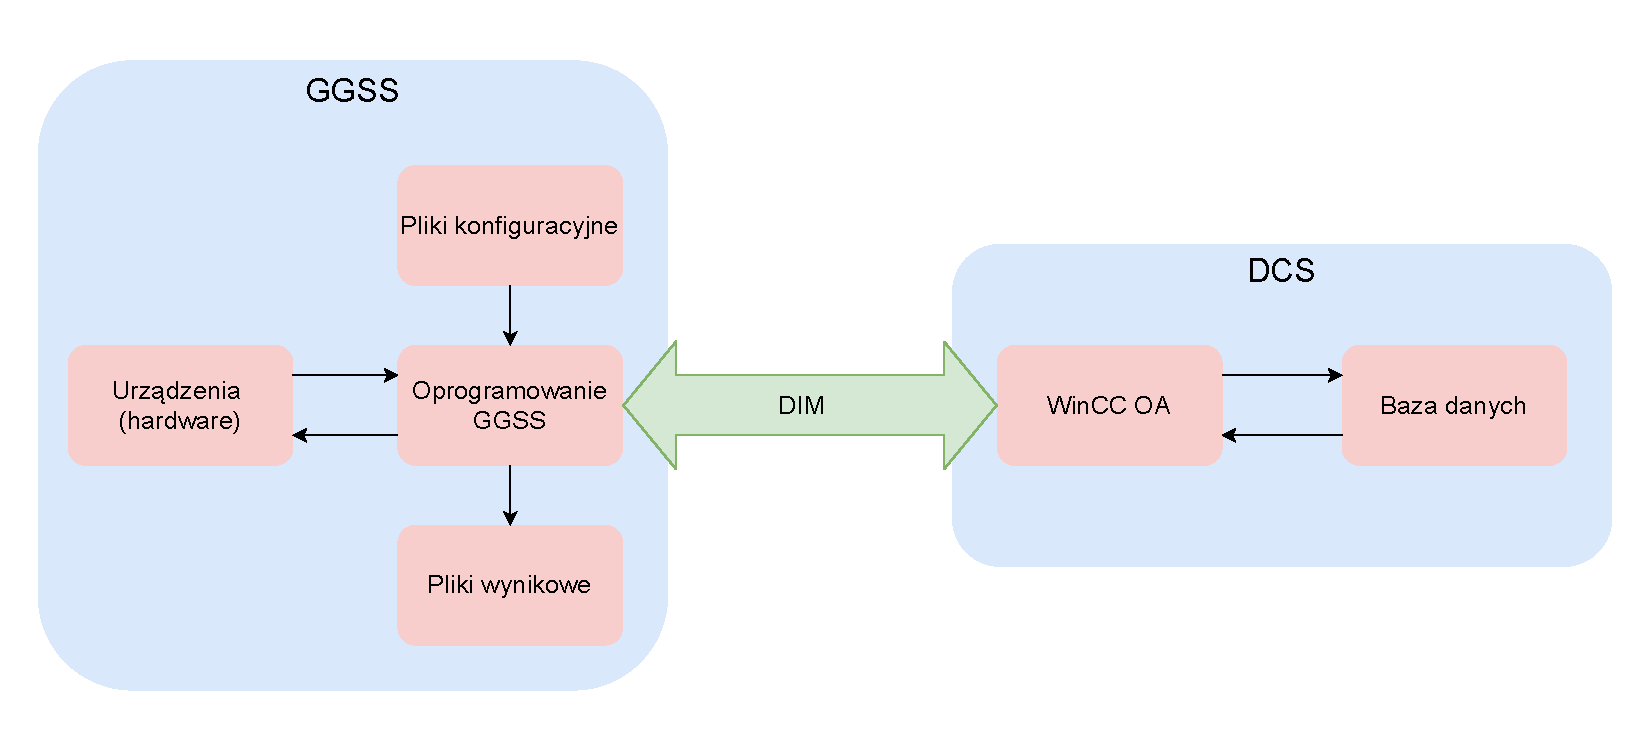
\includegraphics[width=\textwidth]{high_level_architecture.pdf}
\caption{Wysokopoziomowa architektura projektu GGSS. Strzałkami oznaczono przepływ danych pomiędzy poszczególnymi komponentami systemu \cite{GGSS_inz}.}
\label{fig:high_level_architecture}
\end{figure}


Szczegóły działania najważniejszych z~punktu widzenia niniejszej pracy elementów systemu omówione zostaną w~dalszej części tego rozdziału. Znaczna część prac opisanych w~niniejszym manuskrypcie skupiona była na udoskonaleniu warstwy oprogramowania systemu GGSS.


\section{Urządzenia elektroniczne}
Z~punktu widzenia warstwy sprzętowej system GGSS składa się z~zestawu tzw. słomkowych liczników proporcjonalnych \cite{mindur_phd} \cite{GGSS_jinst}, zasilanych za pomocą 4-kanałowych zasilaczy wysokiego napięcia. Sygnały generowane przez liczniki przetwarzane są przez wielokanałowy analizator amplitudy (MCA - \emph{Multi-Channel Analyzer}), natomiast wybór licznika słomkowego używanego do wykonania pomiarów następuje za pomocą 8-kanałowego multipleksera sygnałów analogowych \cite{ZadrozniakInz} \cite{ZadrozniakMgr}. Urządzenia podłączone są do komputera PC, który steruje nimi za pomocą oprogramowania systemu GGSS. W~tabeli \ref{tab:devices} zamieszczone zostało zestawienie informacji na temat wykorzystywanych przez projekt urządzeń. Sposób działania systemu (jego podstawa fizyczna oraz znaczenie przeprowadzanych pomiarów) wykracza poza zakres niniejszej pracy, został natomiast szczegółowo opisany w~pracy \emph{Wybrane zagadnienia związane z~pracą słomkowych liczników proporcjonalnych w~detektorze TRT eksperymentu ATLAS} \cite{mindur_phd}, której autorem jest dr hab. inż. Bartosz Mindur, prof. AGH oraz w publikacji \emph{Gas gain stabilisation in the ATLAS TRT detector} \cite{GGSS_jinst}.

\clearpage

\begin{table*}[htbp]
\centering
\caption{Zestawienie istotnych z~punktu widzenia niniejszej pracy urządzeń wchodzących w~skład systemu GGSS.}
\label{tab:devices}
\begin{tabularx}{\textwidth}{@{}lX@{}}
\toprule
Urządzenie &
Informacje \\
\midrule
4-kanałowy zasilacz wysokiego napięcia & CAEN N1470 \cite{caen_n1470} \\
wielokanałowy analizator amplitudy & CAEN N957 \cite{caen_n957} \\
multiplekser sygnałów analogowych & urządzenie autorstwa pana Pawła Zadrożniaka \cite{ZadrozniakInz}\\
\bottomrule
\end{tabularx}
\end{table*}


\section{Warstwa oprogramowania}
Poprzez warstwę oprogramowania systemu GGSS autorzy rozumieją zarówno zestaw aplikacji napisanych w~języku C++ (standard 11), jak i~otaczającą je infrastrukturę (pomocnicze skrypty, system budowania, testowania i~tworzenia nowych wydań). 


Trzon warstwy oprogramowania projektu GGSS stanowi aplikacja \emph{ggss-runner}, zawierająca logikę odpowiedzialną za komunikację z~systemem za pomocą protokołu DIM, gromadzenie i~walidację danych oraz sterowanie urządzeniami wchodzącymi w~skład warstwy sprzętowej. W~skład systemu wchodzi ponadto szereg pomniejszych aplikacji (niektóre z~nich stanowią element dodany przez autorów niniejszej pracy, zostaną więc omówione ze szczegółami w~dalszych jej częściach):
\begin{itemize}
    \item \emph{ggss-spector} - aplikacja okienkowa służąca do wizualizacji zebranych przez system danych (zapisanych w~plikach wynikowych)
    \item \emph{ggss-reader} - niezależna aplikacja \cite{PodsiadloInz} przeznaczona do wykorzystywania na maszynach deweloperskich, pozwalająca na odtwarzanie działania oprogramowania sterującego GGSS, tzn. wysyłająca do systemu kontroli detektora archiwalne dane z~pominięciem warstwy sprzętowej
    \item \emph{ggss-dim-cs} - aplikacja pozwalająca na prowadzenie interakcji z~systemem poprzez udostępnienie możliwości wysyłania do niego komend za pomocą protokołu DIM
    \item zestaw aplikacji \emph{ggss-hardware-service-apps} - proste narzędzia pozwalające na wykonywanie operacji na wchodzących w~skład systemu urządzaniach, w~tym na wykonywanie testów ich działania. 
\end{itemize}


Projekt GGSS charakteryzuje się ponadto rozbudowaną infrastrukturą, w~której skład wchodzą systemy odpowiedzialne za budowanie projektu, zarządzanie zależnościami zewnętrznymi oraz pomiędzy jego komponentami, automatyzację procesu testowania poszczególnych komponentów oraz automatyzację tworzenia i~wersjonowania wydań. Projekt zawiera ponadto skrypty pomocnicze (napisane przy użyciu popularnych języków skryptowych), pozwalające na zarządzanie systemem w~jego środowisku docelowym. Gruntowna przebudowa infrastruktury systemu GGSS stanowiła temat pracy inżynierskiej autorów. W~dalszej części niniejszego manuskryptu omówione zostaną wprowadzone w~ramach pracy magistersiej rozszerzenia.


\section{Oprogramowanie WinCC OA}
SIMATIC WinCC Open Architecture jest oprogramowaniem typu SCADA firmy SIEMENS służącym do wizualizacji i~sterowania procesami produkcyjnymi. Stanowi ono trzon systemu kontroli detektora ATLAS i~pozwala na monitorowanie i~sterowanie pracą wchodzących w~jego skład podsystemów. WinCC OA pozwala m.in. na tworzenie specjalnych paneli, przedstawiających w~przyjaznej dla użytkownika formie graficznej zebrane dane oraz procesy zachodzące w~monitorowanym systemie - przykład tego typu panelu, obrazujący pracę słomkowych liczników proporcjonalnych wchodzących w~skład warstwy sprzętowej systemu GGSS, przedstawiony został na rysunku \ref{fig:winccoa_panel_example}.

\begin{figure}[H]
\centering
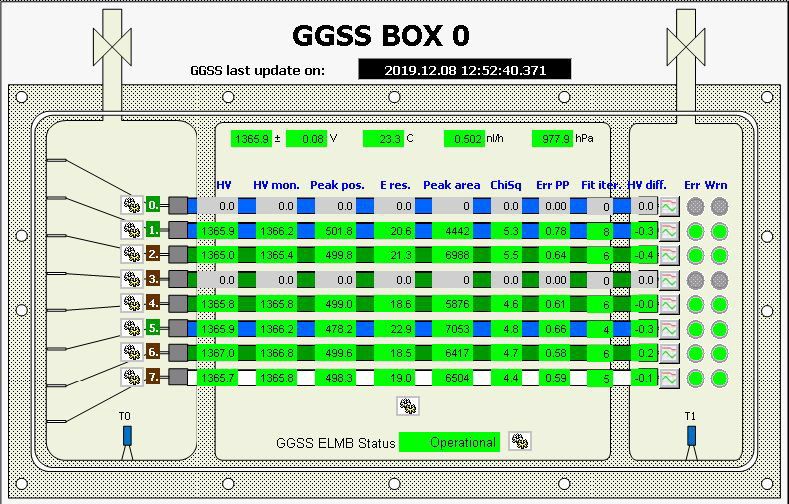
\includegraphics[width=\textwidth]{winccoa_panel.png}
\caption{Fragment przykładowego panelu informacyjno-administracyjnego stworzonego z~wykorzystaniem technologii WinCC OA. Widoczne są m.in.: parametry związane z~pomiarami wykonywanymi za pomocą słomkowych liczników proporcjonalnych (np. \emph{Peak pos.} i~\emph{Peak area}), data ostatniej aktualizacji oraz wskaźniki informujące o~ostrzeżeniach i~błędach.}
\label{fig:winccoa_panel_example}
\end{figure}


Autorzy niniejszego dokumentu nie byli odpowiedzialni za przeprowadzanie prac związanych z~rozwojem oraz utrzymanem systemu WinCC OA funkcjonującego w~ramach infrastruktury CERN. Z~tego też powodu szczegóły jego działania nie zostaną omówione. Istotna, z~punktu widzenia niniejszej pracy, jest natomiast możliwość zastosowania go jako narzędzia ułatwiajacego przeprowadzanie okresowych testów systemu GGSS. Wynika to przede wszystkim z~wygodnej w~użytkowaniu funkcjonalności paneli, pozwalających na monitorowanie działania projektu w~czasie rzeczywistym oraz natychmiastowe wykrywanie wszelkich nieprawidłowości. 


\section{Środowisko docelowe i~ograniczenia}
Charakterystyka środowiska docelowego, w~jakim działa system GGSS, jest z~punktu widzenia niniejszej pracy bardzo istotna, przede wszystkim ze względu na bardzo znaczący związek projektu z~infrastrukturą dostarczaną przez CERN. Stawia to przed autorami szereg ograniczeń dotyczących wersji wykorzystywanych narzędzi, jak również wymusza dodatkowe działania w~przypadku wykonywania pewnych operacji. Do najważniejszych ograniczeń narzucanych przez środowisko docelowe i~specyfikę projektu należą:
\begin{itemize}
    \item dostępna wersja kompilatora języka C++ - w~ramach infrastruktury CERN dostępny jest kompilator \emph{g++ (GCC) 4.8.5}. Wersja ta wspiera w~większości standard C++11, a~zatem funkcjonalności takie jak wyrażenia lambda czy semantyka przenoszenia. Niestety oferowane przez nią wsparcie nie jest pełne - brakuje m.in. poprawnej implementacji biblioteki odpowiedzialnej za przetwarzanie wyrażeń regularnych. Ze względu na wymóg zapewnienia możliwości budowania projektu na maszynie docelowej, ograniczenie to stanowiło znaczące utrudnienie podczas prac nad kodem źródłowym aplikacji wchodzących w~skład systemu.
    \item dostępna wersja narzędzia CMake - na maszynach docelowych dostępna jest wersja \emph{2.8.12.2}, stanowiąca bardzo stare wydanie narzędzia. Oprogramowanie w~znacząco nowszej wersji (tzn. o~numerze wyższym od \emph{3.0}) dostępne jest jedynie na wybranych komputerach wchodzących w~skład infrastruktury CERN, przez co zdecydowano o~pozostaniu przy starym jego wydaniu. Stosowana wersja nie zawiera wielu powszechnie stosowanych współcześnie funkcjonalności oraz charakteryzuje się innym podejściem do zarządzania zależnościami (operacje na poziomie katalogów, uznawane za tzw. \emph{złą praktykę}).
    \item związek projektu z~wersją jądra systemu - jednym z~modułów wchodzących w~skład systemu GGSS jest \emph{ggss-driver}, zawierający sterownik dla wielokanałowego analizatora amplitudy CAEN N957. Istnienie tego modułu wymusza zgodność wersji jądra systemu operacyjnego pomiędzy środowiskiem deweloperskim i~produkcyjnym, co w~konsekwencji prowadzi do komplikacji infrastruktury budowania projektu - konieczne jest stosowanie maszyn wirtualnych oraz narzędzia konteneryzacyjnego Docker podczas procesu budowania komponentu \emph{ggss-driver} (stosowane rozwiązanie opisane zostało przez autorów szczegółowo w~ich pracy inżynierskiej).
    \item ograniczone uprawnienia w~środowisku docelowym - infrastruktura na której uruchamiany jest projekt GGSS jest środowiskiem CERN o~zaostrzonym rygorze. Wszelkie instalowane aplikacje, zmiany w~systemie, bibliotekach, czy też prostych ustawieniach użytkownika muszą być konsultowane z~administratorami systemowymi. Autorzy nie mają możliwości wprowadzania na własną rękę praktycznie żadnych zmian.
    \item możliwość przeprowadzania testów tylko w~określonych momentach prac nad projektem - nad systemami GGSS oraz DCS pracuje wielu ekspertów, testowanie projektu możliwe jest zatem tylko wtedy, gdy nie zakłóca to prac innych osób i~jest fizycznie możliwe (np. gdy nie są wykonywane prace nad warstwą sprzętową systemu). Wymusza to dostosowanie tempa prac w~taki sposób, by jednocześnie testowany był ograniczony, ale znaczący zakres zmian (m.in. by możliwe było szybkie wprowadzenie poprawek w~przypadku wykrycia błędu).
    \item konieczność zachowania kompatybilności wstecznej - zmiany wprowadzane w~systemie nie mogą powodować, że starsze wersje komponentów, z~jakich składa się system GGSS (rys. \ref{fig:high_level_architecture}) staną się niezdatne do użycia, np.: dodanie nowego parametru do pliku konfiguracyjnego nie powinno wykluczać możliwości użycia starszej wersji tegoż pliku oraz starszej wersji oprogramowania. Tego typu ograniczenia obowiązują również w~kontekście danych wymienianych pomiędzy aplikacją GGSS a~systemem kontroli detektora za pomocą protokołu DIM - dane mają odgórnie ustalony, niemożliwy do zmiany format.
\end{itemize}


\chapter{Praktyki stosowane w projekcie} % TODO: nazwa
\label{cha:practices}

Celem tego rozdziału jest opisanie praktyk stosowanych w projekcie GGSS podczas wykonywania pracy magisterskiej. Poruszone zostaną tematy organizacji pracy nad kodem w zespole, dokumentacja projektu, czy też konwencje zastosowane w celu uzyskania jednolitego kodu źródłowego w przestrzenii całego systemu GGSS.

\section{Wprowadzenie do problematyki}
Ze względu na zespołowy charakter w trakcie wykonywania pracy inżynierskiej zostały wprowadzone praktyki mające na celu organizację i koordynację współpracy. W ramach platformy GitLab, wykorzystywanej przez CERN jako główne narzędzie do współpracy nad kodem skorzystano z szeregu funkcjonalności ułatwiających śledzenie postępów, jak i zarządzanie projektem. Oprócz utworzenia zespołu, do którego został przypisany kod projektu oraz w ramach którego odbywała się kolaboracja, wykorzystano:
\begin{itemize}
\item issue - opis pojedynczego zadania/problemu. Zawiera podstawowy informacje, przypisaną osobę, etykietę, która oznacza obecny stan, termin wykonania oraz wagę
\item kanban board - tablica kanban zawierająca wszystkie przypisane do projektu issues. Kolumny takiej tabeli stanowią spersonalizowane do projektu etykiety. Pozwala na wysokopoziomowe zarządzanie projektem, sprawdzenie statusu, czy też łatwą zmianę etykiety przypisanej do zadań poprzez przeciągnięcie do odpowiedniej kolumny.
\item merge request -  dedykowany widok do wprowadzania zmian wprowadzonych w ramach kodu deweloperskiego do kodu produkcyjnego, który jest wykorzystywany do tworzenia i dostarczania aplikacji
\item milestone - jednostka organizacyjna pozwalająca na grupowanie kilku issues, które realizują większy cel opisany w ramach milestone. Milestone śledzi przypisane do niego issues, przewidywany czas zakończenia, wagę pozostałych do wykonania issues.
\end{itemize}
W trakcie wykonywania pracy inżynierskiej, szczególnie podczas początkowego etapu projektu, który odbywał się w trakcie 3-tygodniowego wyjazdu do CERN, wyżej wymienione praktyki sprawdzały się bardzo dobrze.

\section{Motywacja do wprowadzenia zmian}
Ze względu na dobre sprawowanie się wyżej wymienionych praktyk w trakcie pracy inżynierskiej postanowiono na kontynuowanie ich wykorzystania również w trakcie pracy magisterskiej. Z powodu nieregularnego aspektu pracy nad projektem, wykonywanie czynności zdalnie, lepsze poznanie środowiska, wykorzystywanych narzędzi oraz samej platformy GitLab postanowiono dostosować stosowane praktyki do nowych realiów. Dodatkowo bardzo ważną zasadą, biorąc pod uwagę zakończenie pracy nad projektem i przekazanie go osobie odpowiedzialnej za dalsze utrzymanie, było odpowiednie udokumentowanie całego projektu. Wymagało się, aby możliwie proste było wprowadzanie zmian do systemu GGSS oraz sprawne, nieprzerwane działanie po zakończeniu pracy magisterskiej. Dlatego dostarczona dokumentacja musiała być obszerna oraz dobrze opisująca zastosowane rozwiązania. Dodatkowo biorąc pod uwagę mocny nacisk tejże pracy na część aplikacyjną projektu potrzebne było zdefiniowanie pewnych zasad pozwalających na ustandaryzowaną pracę z kodem źródłowym aplikacji. Pozwoliło to na zachowanie pewnych konwencji w całym projekcie, co zapobiegało różnicom w kodzie między komponentami, a co za tym idzie utrzymanie kodu oraz wdrożenie nowych osób do projektu jest znacznie uproszczone.


\section{Zmiana praktyk ze względu na niereguralność prac}

Prace nad systemem GGSS były kontynuowane, z mniejszymi przerwami, od obrony pracy inżynierskiej. Natomiast ich charakter był nieregularny. Każdy z autorów pracował nad systemem w wybranych przez siebie godzinach. Ze względu na to wszystkie praktyki, które opierały się o regularny czas pracy oraz przewidywanie czasu zakończenia danych zadań nie miały większego zastosowania. Postanowiono zatem zaprzestać przypisywania wag poszczególnym zadaniom. Oprócz wartości szacunkowej niewiele ona wnosiła w trakcie wykonywania zadania, dodatkowo przybrane wartości czasami różniły się od rzeczywistej wagi problemu, ponieważ często zadania wymagały w pierwszej kolejności zgłębienia tematu, a następnie określenia dokładnego rozwiązania problemu.

Zarzucono również praktykę wypełniania pola “termin oddania” w ramach tworzonych zadań. Ze względu na  wcześniej wspomniany czas poświęcany na pracę nad projektem, a szczególnie jego regularność, informacja ta często nie sprawdzała się z rzeczywistym czasem zakończenia zadania. Dodatkowo informacja ta nie była praktycznie w ogóle potrzebna w trakcie prac nad projektem ze względu na sposób formułowania zadań, które były możliwe do realizacji bez wpływu na pozostałe zadania - były od siebie niezależne. W przypadku zadań, które wymagały koordynacji, czy też pracy od obydwu autorów, organizowane były spotkania online z wykorzystaniem narzędzi takich jak Microsoft Teams, które pozwalały na tworzenie konferencji podczas których realizowane były wyżej wymienione zadania, czy też określane były ramy czasowe wykonania zadań od siebie zależnych. Sposób ten sprawdził się bardzo dobrze i nie wymagana była dodatkowa koordynacja dla tego typu prac.

Rysunek \ref{fig:issue} przedstawia \emph{issue} utworzone według nowo ustalonych zasad. Brak jest przypisanego \emph{milestone}, czy też \emph{due date}. Natomiast ważne, wartościowe informacje, przydatne w trakcie pracy nad projektem są wypełnione, tj.: rozbudowany opis pozwalający w krótkim czasie zrozumieć o co chodzi w konkretnym zadaniu, osoby przypisane do \emph{issue} oraz etykiety oznaczające aktualny stan wykonania zadania, czy też jakikolwiek powód z którego \emph{issue} nie zostało, bądź nie zostanie wykonane.

\begin{figure}[H]
    \centering
    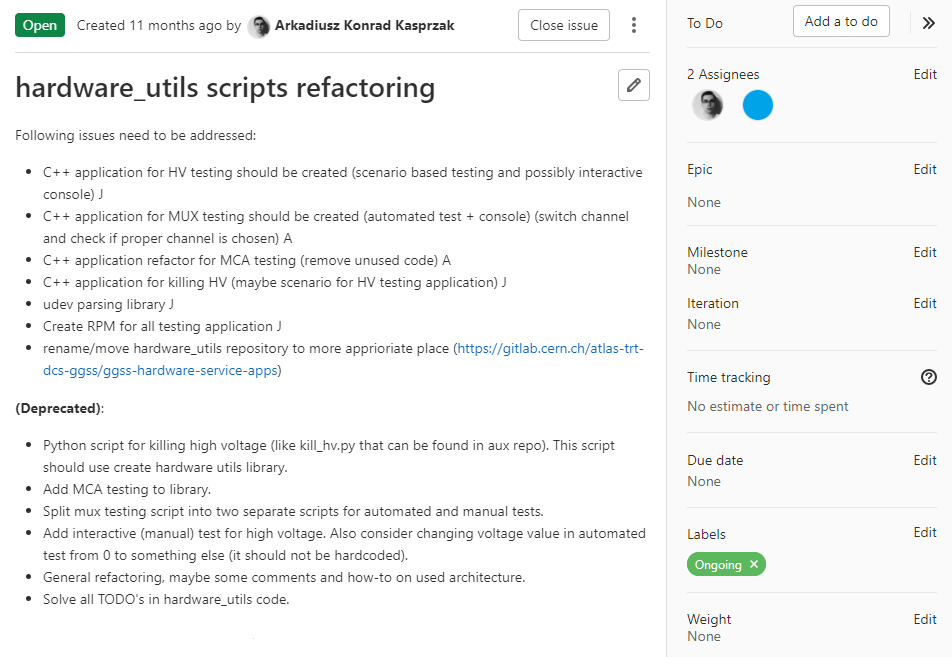
\includegraphics[width=\textwidth]{components/practices_res/issue}
    \caption{Przykładowe \emph{issue} wg. nowo przyjętych praktyk}
    \label{fig:issue}
\end{figure}


\newpage
\section{Dokumentacja projektu}

%Wstepny tekst
Projekt GGSS ma być utrzymywany i pozostać w użyciu również po zakończeniu działań nad pracą dyplomową. Ze względu na to że rozwiązania wprowadzone do projektu były zarówno implementowane, jak i projektowane przez autorów w porozumieniu z promotorem, posiadają oni niezbedną do uwiecznienia wiedzę nt.: powodów zastosowania pewnych rozwiązań, sposobu ich działania, sposobu korzystania z nich, czy też zasad, które należy stosować w trakcie rozwoju aplikacji. Ze względu na te czynniki dużo uwagi poświęcono przygotowaniu odpowiedniej dokumentacji pozwalającej na swobodną pracę z projektem przez osoby, które ten projekt będą nadal utrzymywać.

% Dokumentacja na poziomie README
Dokumentacja w postaci plików \emph{README} napisanych w języku znaczników \emph{Markdown} jest dedykowana dla każdego z repozytoriów. Zazwyczaj opisana jest w niej zawartość danego repozytorium, sposób użycia tejże zawartości, jeżeli wcześniejsze przygotowanie zawartości jest potrzbne opisane są kroki, które należy w takiej sytuacji poczynić. Dodatkowo w wyżej wymienionych plikach opisane są wszelkie niuanse, czy też bardziej zaawansowane kwestie dotyczące zawartości danego repozytorium.

Rysunek \ref{fig:readme} przedstawia przykładowy plik \emph{README} dla repozytorium \emph{ggss-all} zawierające infrastrukturę do budowy głównej aplikacji systemu GGSS. Wyżej wymieniony plik zawiera informacje o przeznaczeniu repozytorium, wymaganiach potrzebnych do spełnienia w celu uruchomienia infrastruktury budującej aplikację, krokach które należy podjąć, aby skorzystać z tejże infrasturktury. Oprócz tego plik ten zawiera gotowe do użycia komendy, które można skopiować i wkleić bezpośrednio do konsoli w celu skorzystania z infrastruktury. Plik ten zawiera również, a co nie jest widoczne na rysunku, informacje o sposobie uzyskania dostępu do kodu protokołu DIM, który jest wymagany do działania systemu GGSS.


Przygotowana w ten sposób dokumentacja pozwala osobie praktycznie niezapoznanej z projektem na skorzystanie z infrastruktury i przygotowanie gotowej do użycia, w środowisku docelowym, aplikacji. Również powrót do projektu po dłuższej przerwie nie powinien powodować większych trudności.
\newpage
\begin{figure}[H]
    \centering
    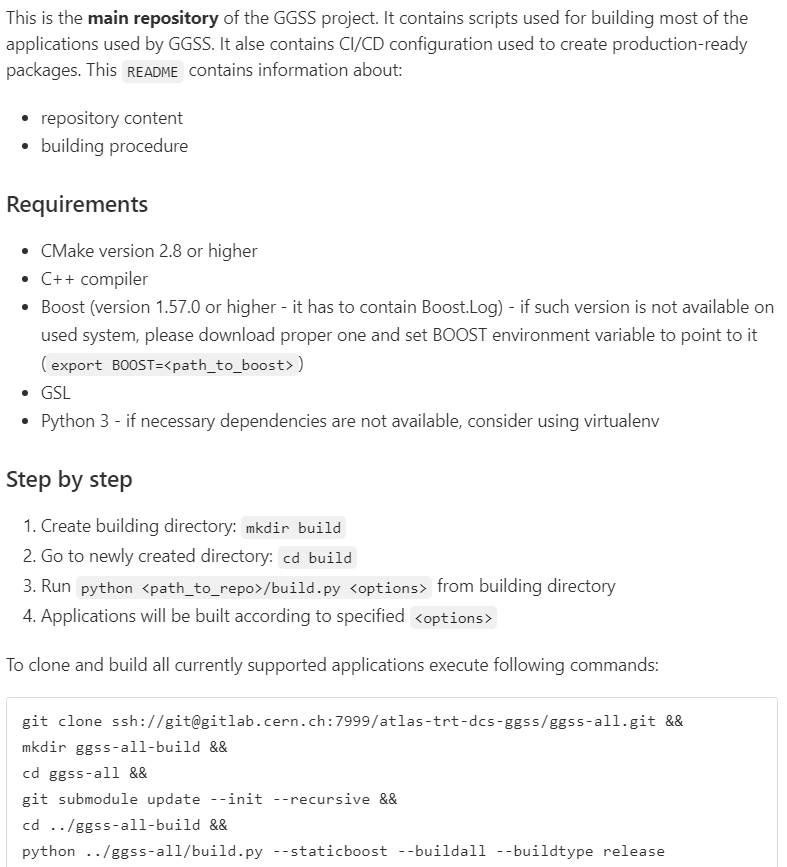
\includegraphics[width=\textwidth]{components/practices_res/readme}
    \caption{Przykładowe \emph{README} w ramach repozytorium \emph{ggss-all}}
    \label{fig:readme}
\end{figure} % zembedowac pdf

% Dokumentacja na poziomie kodu źrółowego
W projekcie została zastosowana również dokumentacja na poziomie kodu źródłowego. Znajduje się ona między innymi: przed klasami, przed metodami, czy też na początku plików źródłowych. Dokumentacja ta stosuje format zgodny z narzędziem \emph{doxygen}, co pozwaliło na jej ujednolicenie i zwiększenie czytelności. Dzięki wcześniej wspomnianej zgodności możliwe jest wygenerowanie dokumentacji w postaci plików \emph{html}. Dokumentacja taka, w celu jej przeczytania, wymaga jedynie aktualnej przeglądarki internetowej. W celu pełnego wsparcia dokumentacji w postaci plików \emph{html} generowanych z użyciem narzędzia \emph{doxygen} potrzebne było również dostosowanie infrastruktury służącej do budowania projektu, a dokładnie plików \emph{CMake}, dzięki czemu wygenerowane pliki \emph{make} posiadają moduły odpowiedzialne za obsługę wcześniej wspomnianej dokumentacji.

Rysunek \ref{fig:code_documentation} przedstawia przykładową dokumentację zgodną z formatem wspieranym przez narzędzie \emph{doxygen}. Zawiera ona krótki opis dotyczący metody, następnie opis każdego z parametrów przyjmowanych przez daną metodą oraz wartość zwracaną przez metodę. Informacje te są bardzo przydatne w przypadku, gdy nie jesteśmy pewni, zważając na samą definicję metody, jej działania, parametrów wejściowych, czy też wyjścia. Opis taki rozwiewa częściowo wątpliwości i pozwala w poprawny sposób skorzystać z wcześniej napisanego kodu.
\begin{figure}[H]
    \centering
    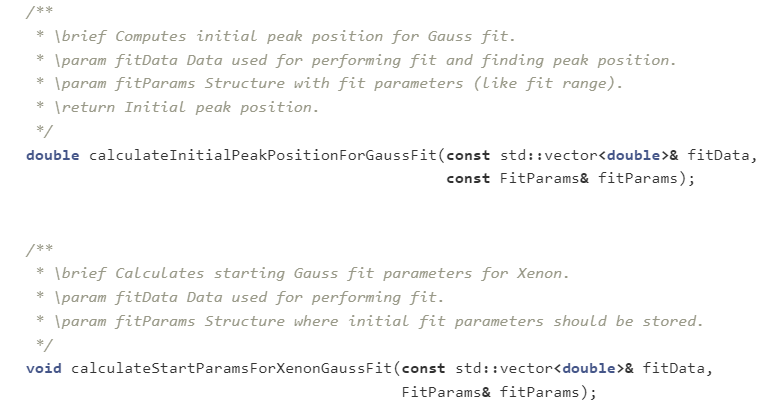
\includegraphics[width=\textwidth]{components/practices_res/code_documentation}
    \caption{Przykładowa dokumentacja metod w bibliotece \emph{fit-lib} w ramach projektu GGSS}
    \label{fig:code_documentation}
\end{figure} % wstawic jako listing

Rysunek \ref{fig:doxygen} przedstawia dokumentację jednej z metod w bibliotece \emph{log-lib}. Zawartość jest zbliżona jak w przypadku rysunku \ref{fig:code_documentation}, natomiast przedstawiona w bardziej przystępny sposób. Dokumentacja wygenerowana za pomocą narzędzia \emph{doxygen} świetnie nadaje się na udostępnienie zewnętrznym użytkownikom. Pozwala również w łatwiejszy sposób przeglądać pełną dokumentację danego modułu bez potrzeby przeglądania kodu źrodłowego.

\begin{figure}[H]
    \centering
    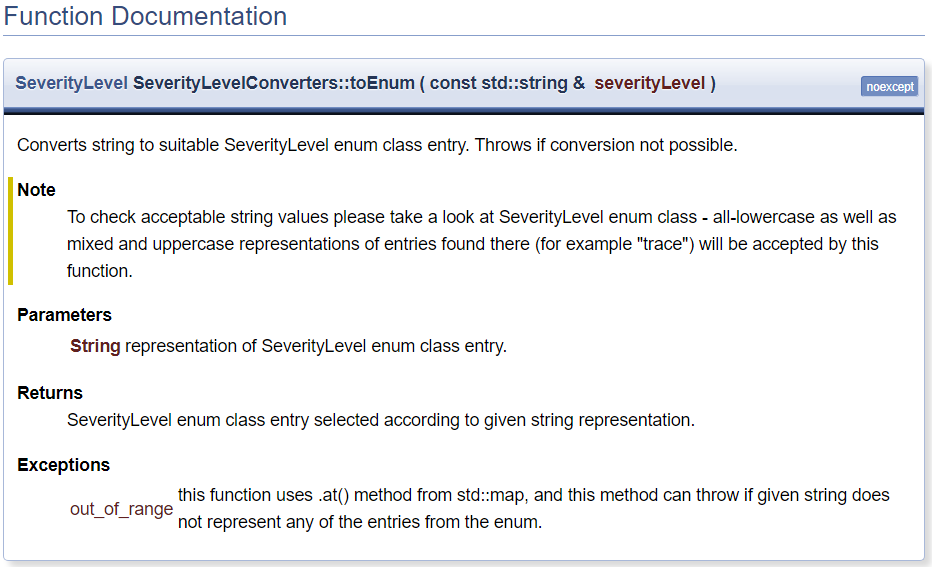
\includegraphics[width=\textwidth]{components/practices_res/doxygen}
    \caption{Przykładowa dokumentacja metod w bibliotece \emph{fit-lib} w ramach projektu GGSS}
    \label{fig:doxygen}
\end{figure}

Ostatnim elementem dokumentacji zawartym w projekcie są dokumenty \emph{how-to}. Napisane, podobnie jak pliki \emph{README}, za pomocą języka znaczników \emph{Markdown}, natomiast mają charakter globalny dla całego projektu - nie ograniczają się do jednego repozytorium. Dokumenty takie znajdują się w repozytorium \emph{ggss-aux}. Opisane są tam krok po kroku bardziej zaawansowane aspekty pracy z projektem GGSS, jak np.: sposób obsługi architektury wielo-poziomowej opartej o submoduły, czy też przygotowywanie wirtualnej maszyny do pracy jako \emph{gitlab runner} w środowisku GitLab udostępnionym w ramach infrastruktury CERN.

\section{Konwencja kodowania}


Ze względu na to, że w trakcie pracy magisterskiej bardzo duży nacisk położono na część aplikacyjną projektu autorzy, jeszcze przed rozpoczęciem pracy nad kodem źródłowym, postanowili ustanowić konwencję kodowania, tak, aby na przestrzenii całego projektu GGSS utrzymać jednolity kod. Zasady, które zostały ustalony tyczą się nazewnictwa: klas, przestrzenii nazw, zmiennych, plików. Postanowiono wykorzystać, dobrze znane w środowisku, systemy notacji ciągów tekstowych \emph{lower camel case} oraz \emph{upper camel case}. Ze względu na różnorodność możliwych rozszerzeń plików w przypadku języka C++ postanowiono również ujednolicić ten aspekt. W przypadku plików z kodem źródłowym zastosowano rozszerzenia \emph{.cpp} oraz \emph{.h}.

Ustanawiając konwencję kodowania postanowiono ograniczyć się do wyżej wymienionych aspektów, sposób projektowania architektury, podziału na foldery, klasy, etc. wewnątrz danego modułu pozostawiono bez większych obostrzeń. Oczywiście autorzy w każdym z dotkniętych miejsc stosowali dobre praktyki progrmaistyczne oraz tak zwany \emph{clean code}, natomiast, ze względu na to, że w większości przypadków prace nad projektem dotyczyły modyfikacji już istniejącego kodu oraz modułów była zachowana wcześniej zastosowana architektura.


\chapter{Prace nad architekturą i infrastrukturą projektu}
\label{cha:infra}


Niniejszy rozdział zawiera opis prac wykonanych przez autorów w ramach rozwoju architektury i infrastruktury systemu GGSS. Rozdział ten stanowi bezpośrednią kontynuację pracy inżynierskiej autorów, gdzie przygotowane zostały pierwsze wersje rozwijanych w ramach pracy magisterskiej rozwiązań. Przedstawione tu informację dotyczą szerokiego zakresu zagadnień związanych z inżynierią oprogramowania, takich jak: zarządzanie strukturą projektu oraz jego zależnościami, automatyzacja procesów towarzyszących wytwarzaniu oprogramowania czy przygotowanie infrastruktury ułatwiającej testy warstwy sprzętowej systemu. 

\section{Zmiany w architekturze projektu}
Przez zmiany w architekturze projektu autorzy rozumieją stopniowy rozwój rozwiązania przygotowanego w ramach napisanej przez nich pracy inżynierskiej. Wprowadzone po jej zakończeniu modyfikacje to przede wszystkim uproszczenie powstałej hierarchii zależności między poszczególnymi elementami warstwy oprogramowania (rozumianymi zarówno jako repozytoria, jak i biblioteki), uczynienie systemu bardziej przystępnym dla użytkownika (np. poprzez nadanie komponentom nazw dobrze oddających ich przeznaczenie) oraz przygotowanie systemu pozwalającego w prosty sposób odtworzyć kod źródłowy w wersji bez wprowadzonych w ramach pracy magisterskiej modyfikacji (jako rodzaj zabezpieczenia przed skutkami potencjalnych błędów, które mogły zostać wprowadzone do oprogramowania podczas prac nad nim). Znaczna część zmian opisanych w niniejszej części pracy była możliwa do wprowadzenia z uwagi na trwające jednocześnie prace nad kodem źródłowym systemu GGSS i zmiany zachodzące w ich czasie. 


\subsection{Początkowa architektura projektu}
Przeprowadzone przez autorów w ramach pracy inżynierskiej modyfikacje architektury systemu GGSS obejmowały przede wszystkim migrację projektu do systemu kontroli wersji Git, wprowadzenie spójnego nazewnictwa poszczególnych komponentów oraz zastosowanie funkcjonalności submodułów będącej częścią technologii Git do stworzenia hierarchicznej struktury repozytoriów (w odróżnieniu od pierwotnej, płaskiej architektury opartej o katalogi). Celem tych zmian było ułatwienie pracy nad pojedynczymi komponentami projektu oraz uczynienie struktury projektu przyjazną dla użytkownika, co zostało zdaniem autorów osiągnięte. 

Architektura stanowiąca punkt wyjściowy zmian wykonanych w ramach niniejszej pracy przedstawiona została na rysunku \ref{fig:old_structure} (z pominięciem repozytoriów pomocniczych, zawierających np. dokumentację). Projekt składał się więc pierwotnie z 14 repozytoriów zawierających wchodzące w skład oprogramowania systemu GGSS biblioteki, aplikacje i skrypty. Przygotowane w ten sposób rozwiązanie charakteryzowało się jednak pewnymi wadami i ograniczeniami, z których najważniejsze to:
\begin{itemize}
    \item głęboka hierarchia zależności, mająca negatywny wpływ na wydajność działania mechanizmu submodułów
    \item istnienie repozytorium \emph{ggss-misc}, zawierającego (poza szablonami CMake) elementy kodu źródłowego niepasujące do pozostałych bibliotek wchodzących w skład systemu: bazowe klasy wyjątków stosowanych w całym projekcie oraz flagi konfigurujące projekt w zależności od systemu operacyjnego (konieczność zastosowania tego typu zabiegu wynikła wprost z założenia o niemodyfikowaniu kodu źródłowego w czasie tworzenia pracy inżynierskiej)
    \item zachowanie oryginalnych nazw bibliotek i aplikacji, dostosowując je jedynie do przyjętej konwencji. Jedną z bibliotek wchodzących w skład projektu była biblioteka statyczna \emph{handle-lib}, odpowiedzialna za implementację mechanizmu slotów i sygnałów (\textbf{pisownia}), na co, zdaniem autorów, jej nazwa nie wskazuje.
    \item wnioskowanie o zależnościach pomiędzy bibliotekami na podstawie dyrektyw preprocesora \emph{include} zawartych w kodzie źródłowym, a nie wykorzystywanych funkcjonalności, co wynikało z niewielkiego doświadczenia i wiedzy autorów na temat systemu podczas tworzenia pracy inżynierskiej oraz wspomnianego już założenia o niemodyfikowaniu kodu źródłowego.
    \item założenie o tworzeniu oddzielnego repozytorium dla każdej z występujących w projekcie aplikacji, niezależnie od jej rozmiarów, co ostatecznie znacznie skomplikowało powiązania pomiędzy repozytoriami (np. repozytoria \emph{external-caen-n957-demo} oraz \emph{mca-n957} charakteryzują się podobnymi zależnościami i oba zawierają niewielkie aplikacje, których zadaniem jest współpraca z wielokanałowym analizatorem amplitudy CAEN N957 - mogłoby być więc połączone w jedno repozytorium).
    \item brak łatwego sposobu na odtworzenie pierwotnej postaci kodu źródłowego - mechanizm ten nie był potrzebny na etapie pracy inżynierskiej, ponieważ nie dokonywano wtedy modyfikacji we wspomnianym kodzie.
\end{itemize}

\begin{landscape}

\begin{figure}[H]
\centering
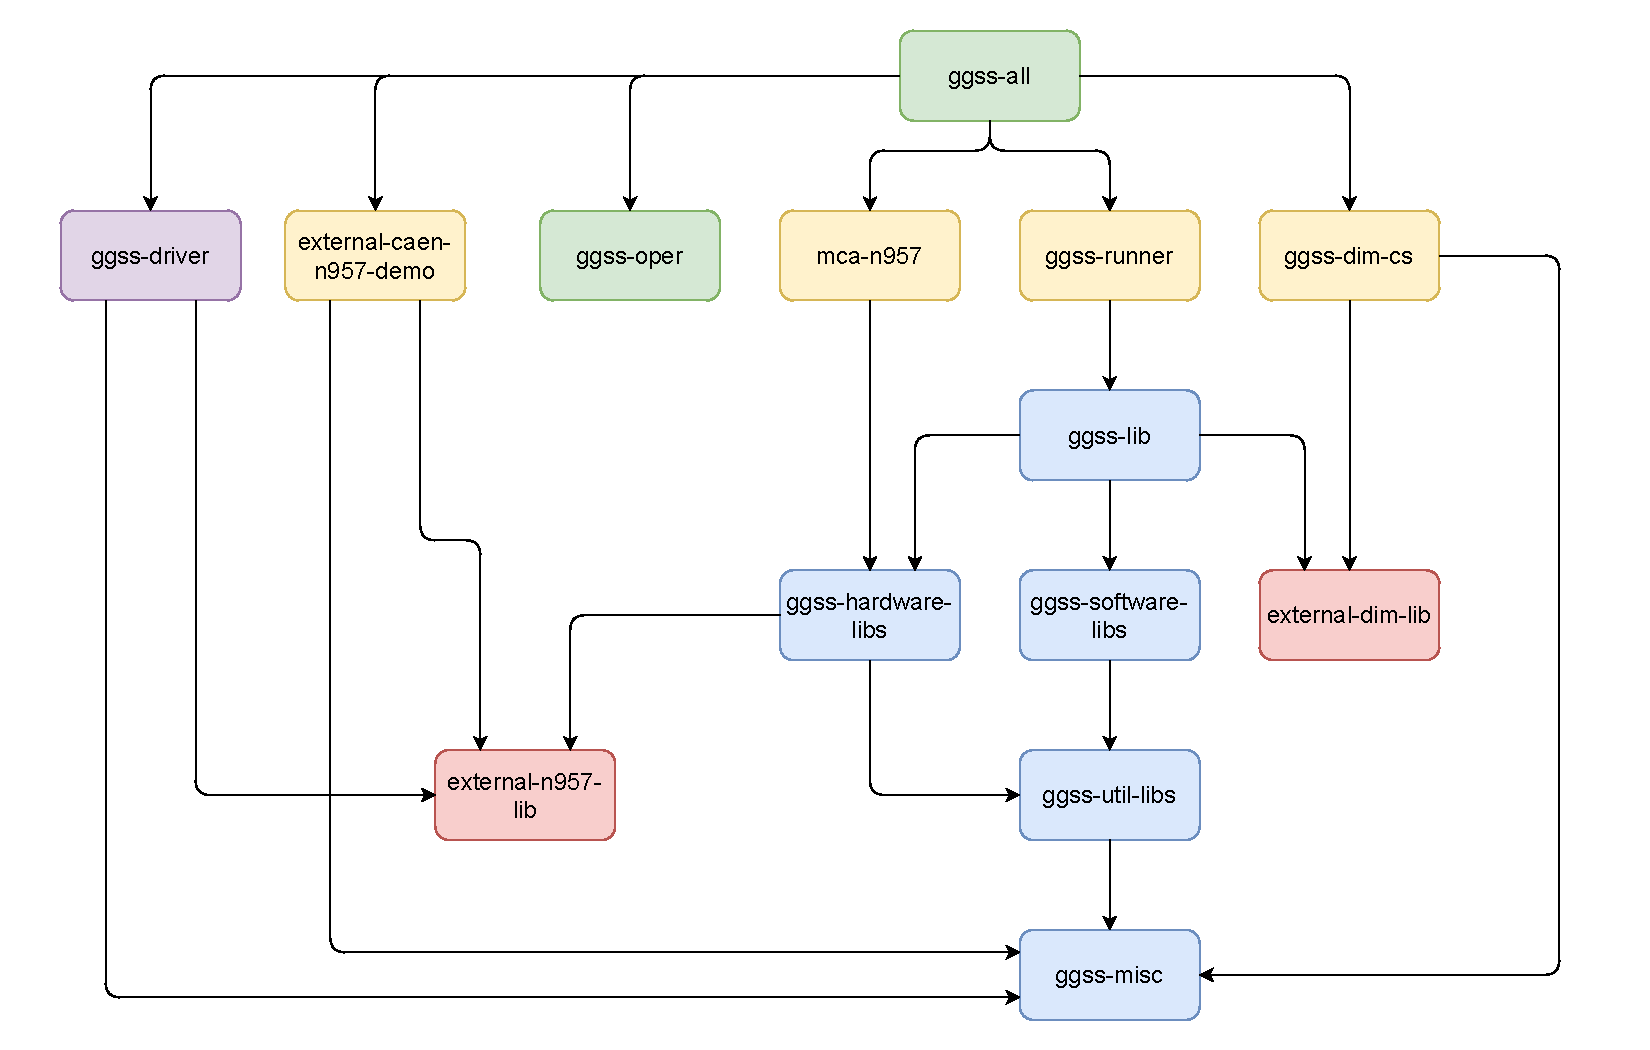
\includegraphics[width=1.4\textwidth]{components/infra_images/old_structure.pdf}
\caption{}
\label{fig:old_structure}
\end{figure}

\end{landscape}

\subsection{Uproszczenie architektury projektu}
Pierwszym podjętym przez autorów działaniem mającym na celu modyfikację struktury projektu była próba jej uproszczenia poprzez analizę zależności wewnętrzych systemu (tzn. zależności pomiędzy poszczególnymi bibliotekami). Należy tutaj zwrócić uwagę, że prac tych nie wykonywano przez pierwsze pół roku od rozpoczęcia przez autorów studiów magisterskich - skupienie się na użytkowaniu stworzonej architektury pozwoliło autorom zarówno na zapoznanie się lepiej z projektem, jak również na samodzielną obserwację jej zalet i wad. 

W celu zrozumienia wprowadzonych w projekcie zmian, konieczne jest zrozumienie toku rozumowania, jakim posługiwali się autorzy pracy podczas tworzenia oryginalnej struktury projektu - dotyczy to przede wszystkim repozytoriów \emph{ggss-lib}, \emph{ggss-software-libs}, \emph{ggss-hardware-libs}, \emph{ggss-util-libs} oraz \emph{ggss-misc}. Ich rola w projekcie prezentuje się następująco:
\begin{itemize}
    \item \emph{ggss-hardware-libs} - przechowywanie bibliotek odpowiedzialnych za obsługę urządzeń wchodzących w skład warstwy sprzętowej systemu GGSS. W pierwotnej wersji projektu były to następujące biblioteki:
    \begin{itemize}
        \item \emph{caenhv-lib} oraz \emph{caenn1470-lib} - odpowiedzialne za komunikację z zasilaczami wysokiego napięcia CAEN N1470
        \item \emph{mca-lib} oraz \emph{ortecmcb-lib} - odpowiedzialne za obsługę wielokanałowego analizatora amplitudy CAEN N957
        \item \emph{usbrm-lib} - odpowiedzialna za obsługę multipleksera sygnałów analogowych
    \end{itemize}
    \item \emph{ggss-software-libs} - przechowywanie bibliotek odpowiedzialnych za implementację wykorzystywanych przez system algorytmów i struktur danych związanych ściśle z warstwą oprogramowania (tzn. nie mających związku z warstwą sprzętową). W pierwotnej wersji projektu były to następujące biblioteki:
    \begin{itemize}
        \item \emph{xml-lib}
        \item \emph{fifo-lib}
        \item \emph{fit-lib}
        \item \emph{daemon-lib}
    \end{itemize}
    \item \emph{ggss-util-libs} - przechowywanie bibliotek, od których zależne są zarówno komponenty odpowiedzialne za obsługę warstwy sprzętowej projektu, jak i związane wyłącznie z warstwą oprogramowania. Innymi słowy, są to biblioteki nie mogące znaleźć się w żadnym z dwóch wymienionych powyżej repozytoriów. W pierwotnej wersji projektu były to:
    \begin{itemize}
        \item \emph{log-lib}
        \item \emph{utils-lib}
        \item \emph{handle-lib}
        \item \emph{thread-lib}
    \end{itemize}
    \item \emph{ggss-misc} - 
    \item \emph{ggss-lib} - przechowywanie kodu źródłowego zawierającego główną logikę systemu GGSS
\end{itemize}

Prace nad kodem źródłowym projektu pozwoliły autorom zaobserwować, iż pewna część występujących w nim dyrektyw preprocesora \emph{include} nie oddaje w poprawny sposób faktycznej struktury zależności między bibliotekami. Najważniejszy przykład stanowi łańcuch zależności występujących pomiędzy biblioteką \emph{ggss-lib}, a bibliotekami \emph{caenhv-lib} oraz \emph{thread-lib}. W oryginalnej wersji projektu zależności między wymienionymi komponentami prezentowały się tak, jak na rysunku \ref{fig:dependency_problem_old}, tzn. bibliteka \emph{ggss-lib} zależna była od biblioteki \emph{caenhv-lib}, która natomiast zawierała dyrektywę \emph{include} dołączającą plik nagłówkowy z biblioteki \emph{thread-lib}. 


\savebox{\mybox}{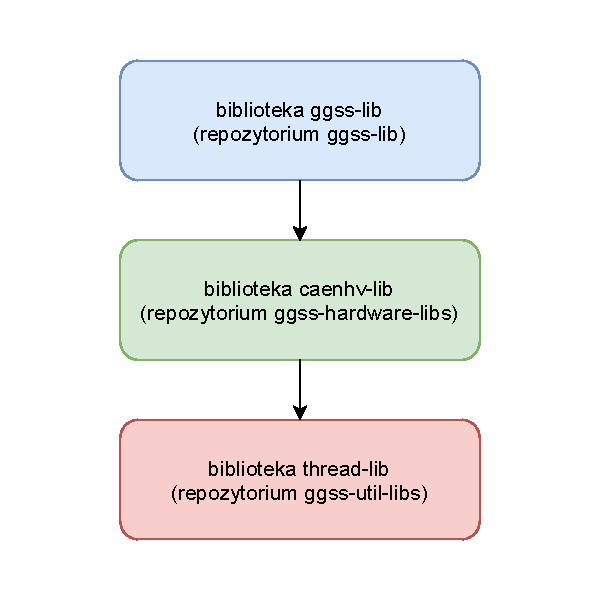
\includegraphics[width=0.40\textwidth]{components/infra_images/dependency_problem_old.pdf}}

\begin{figure}[H]
\centering
\begin{subfigure}[t]{0.40\textwidth}
\centering
\usebox{\mybox}
\caption{Test}
\label{fig:dependency_problem_old}
\end{subfigure}
\hfill
\begin{subfigure}[t]{0.55\textwidth}
\centering
\vbox to \ht\mybox{%
    \vfill
    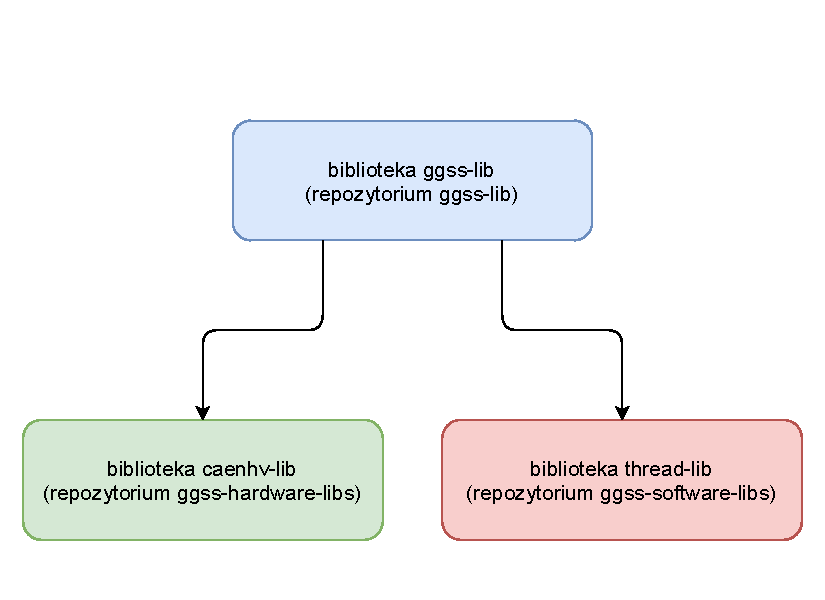
\includegraphics[width=\textwidth]{components/infra_images/dependency_problem_solution.pdf}
    \vfill
}
\caption{Test}
\label{fig:dependency_problem_solved}
\end{subfigure}

\caption{Test}
\end{figure}

W rzeczywistości biblioteka \emph{caenhv-lib} nie wykorzystywała zawartości wspomnianego pliku nagłówkowego - pełniła jedynie formę swego rodzaju pośrednika, udostępniając znajdujące się tam klasy bibliotece \emph{ggss-lib}. Przeniesienie dyrektywy \emph{include} do biblioteki \emph{ggss-lib} spowodowało, iż żadna z bibliotek wchodzących w skład repozytorium \emph{ggss-hardware-libs} nie zawierała zależności do biblioteki \emph{thread-lib}. Rozwiązanie to pozwoliło dokonać migracji tejże biblioteki, wraz z wykorzystywaną przez nią biblioteką \emph{handle-lib}, do repozytorium \emph{ggss-software-libs}, redukując tym samym liczbę bibliotek znajdujących się w repozytorium \emph{ggss-util-libs}. Rysunek \ref{fig:dependency_problem_solved} przedstawia w sposób schematyczny strukturę otrzymanego rozwiązania.

W związku z opisanymi powyżej zmianami ilość kodu źródłowego znajdującego się w repozytorium \emph{ggss-util-libs} znacznie spadła - pozostałe tam biblioteki \emph{log-lib} oraz \emph{utils-lib} charakteryzowały się niewielkim rozmiarem. Spowodowało to, iż jednoczesne istnienie modułów \emph{ggss-misc} oraz \emph{ggss-util-libs} (po wprowadzonych zmianach spełniających tą samą rolę przechowywania niewielkiej liczby komponentów wykorzystywanych przez wiele modułów projektu GGSS) przestało być uzasadnione. Kolejny etap wykonanych prac stanowiło więc przeprowadzenie integracji tychże repozytoriów - w tym celu zdecydowano się na likwidację modułu \emph{ggss-misc} po wcześniejszym przeniesieniu jego zawartości do \emph{ggss-util-libs}.

Migracja znajdujących się w repozytorium \emph{ggss-misc} plików \emph{.cmake} (modułów wykorzystywanych przez infrastrukturę budowania projektu) wymagała, poza wykonaniem trywialnej czynności przeniesienia katalogu, aktualizacji (na poziomie całego projektu) ścieżek wskazujących lokalizację tychże plików. Działanie to było konieczne, ponieważ narzędzie CMake wymaga od programisty, by wyspecyfikował on lokalizację modułów \emph{.cmake} dołączanych do projektu (np. za pomocą komendy \lstinline{include()}) poprzez dodanie ścieżki z ich lokalizacją do listy \lstinline{CMAKE_MODULE_PATH} (przykład wykorzystania tejże listy przedstawiony został na listingu \textbf{listing}). Oznaczało to więc konieczność wykonania, w każdym module wykorzystującym pliki \emph{.cmake}, zmiany wspomnianej ścieżki tak, by wskazywała na katalog \emph{cmake-templates} w repozytorium \emph{ggss-util-libs}.

Poza wspomnianymi plikami \emph{.cmake} w repozytorium \emph{ggss-misc} znajdował się katalog \emph{include}, zawierający trzy pliki nagłówkowe z kodem napisanym w języku C++:
\begin{itemize}
    \item pliki \lstinline{ggssExceptions.h} oraz \lstinline{HardwareException.h} zawierające klasy bazowe wyjątków wykorzystywanych w całym projekcie GGSS
    \item plik \lstinline{CompatibilityFlags.h}, zawierający flagi konfigurujące projekt w zależności od platformy docelowej (Windows lub Linux)
\end{itemize}
Pliki te nie wchodziły oryginalnie w skład żadnej z bibliotek projektu GGSS, nie mogły zostać do nich również dodane przez autorów podczas przygotowywania pracy inżynierskiej, ponieważ wymagałoby to modyfikacji kodu źródłowego systemu. Podczas przeprowadzanej w ramach niniejszej pracy migracji tych plików do repozytorium \emph{ggss-util-libs} zdecydowano się na likwidację katalogu \emph{include} i rozdysponowanie jego zawartości do istniejących lub nowych bibliotek. Plik \lstinline{CompatibilityFlags.h} przeniesiony został więc do biblioteki \emph{utils-lib}, natomiast na potrzebę dwóch pozostałych nagłówków przygotowana została nowa biblioteka \emph{exceptions-lib}. 

Finalna struktura repozytorium \emph{ggss-util-libs} przedstawiona została na listingu \textbf{listing}. Poza wspomnianymi do tej pory zmianami nowość stanowi katalog \lstinline{doxygen-config}, zawierający prosty plik konfigurujący działanie narzędzia Doxygen \textbf{cytat} służącego do generowania dokumentacji programów napisanych w języku C++. Rozszerzenie projektu o możliwość generowania dokumentacji zostanie jednak opisane szczegółowo w dalszej części pracy (sekcja \textbf{dodac referencje do sekcji}).


Poza wspomnianymi do tej pory repozytoriami zmianami objęte zostały ponadto moduły przechowujące aplikacje służące do testowania i obsługi urządzeń elektronicznych wchodzących w skład warstwy sprzętowej systemu GGSS. Motywacją do wprowadzenia modyfikacji była konieczność rozbudowy projektu o kolejne tego typu aplikacje (co zostanie szerzej opisane w sekcji \textbf{sekcja}) - tworzenie dla każdej z nich osobnego repozytorium znacząco komplikowałoby strukturę projektu. Zdecydowano zatem, iż repozytoria \emph{mca-n957} oraz \emph{external-caen-n957-demo} zostaną dołączone do nowo powstałego repozytorium \emph{ggss-hardware-service-apps}, grupującego niewielkie programy służące do operowania na urządzeniach.


% TODO: moze wspomniec o koniecznosci zachowania historii i jak zostało to zrobione???

Poza zmniejszeniem progu wejścia do projektu poprzez uczynienie jego struktury prostszą, opisane do tej pory zmiany korzystnie wpłynęły na działanie mechanizmu submodułów systemu Git, na którym oparty został proces zarządzania zależnościami między repozytoriami w projekcie. Redukcja liczby repozytoriów i powiązań między nimi oraz zmniejszenie głębokości drzewa zależności (poprzez likwidację repozytorium \emph{ggss-misc}) miało pozytywny wpływ na wydajność systemu zarządzającego architekturą projektu. 



\subsection{Dodanie możliwości odtworzenia pierwotnej wersji kodu źródłowego}
% branche legacy, dokumentacja

\subsection{Pomniejsze zmiany}
Poza do tej pory opisanymi, wykonanych zostało kilka pomniejszych modyfikacji mających na celu szeroko pojętą poprawę jakości struktury projektu. Przeprowadzone prace obejmują bogaty zakres wprowadzonych zmian, nie jest więc możliwe zamieszczenie w niniejszej pracy dokładnego opisu każdej z nich. Poniżej krotko opisane zostały więc trzy wybrane przez autorów modyfikacje, charakteryzujące się różnym poziomem skomplikowania, ale operujące na poziomie pojedynczych repozytoriów. 

\subsubsection{Likwidacja repozytorium \emph{ggss-oper}}
Jednym z repozytoriów wprowadzonych przez autorów w ramach wykonywania pracy inżynierskiej był moduł \emph{ggss-oper}, zawierający skrypty oraz pliki konfiguracyjne stanowiące znaczną część infrastruktury przeznaczonej do użytkowania wraz z oprogramowaniem GGSS na maszynie docelowej. Zawartość tego repozytorium, nie stanowiąca wkładu wniesionego przez autorów niniejszej pracy w system, obejmowała m.in.: 
\begin{itemize}
    \item pierwsze wersje skryptów służących do przeprowadzania testów urządzeń wchodzących w skład warstwy sprzętowej projektu (napisane z wykorzystaniem języka Python)
    \item skrypty zarządzające stanem środowiska docelowego (np. ustawiające wymagane zmienne środowiskowe)
    \item skrypty zarządzające oprogramowaniem systemu GGSS, np. \emph{ggss\_monitor.sh} pozwalający na uruchamianie, zatrzymywanie oraz sprawdzanie stanu aplikacji \emph{ggss-runner}
\end{itemize}
Wraz z postępami prac nad projektem, część z wymienionej powyżej zawartości zastąpiona została przez autorów pracy rozwiązaniami alternatywnymi (np. skrypty służące do przeprowadzania operacji na urządzeniach zastąpione zostały aplikacjami napisanymi w języku C++), pozostałe przeniesione zostały natomiast do repozytorium \emph{ggss-all}. Ostatecznie moduł został więc zlikwidowany.


\subsubsection{Utworzenie biblioteki \emph{asyncserial-lib}}
Podczas prac nad kodem źródłowym bibliotek statycznych wchodzących w skład repozytorium \emph{ggss-hardware-libs} zaobserwowano, że w katalogach bibliotek \emph{usbrm-lib} oraz \emph{caenn1470-lib} zamieszczony został, poza właściwym dla nich kodem źródłowym, zestaw plików zawierających implementację asynchronicznej komunikacji z urządzeniami za pomocą interfejsu szeregowego. Ponieważ znalezione w obu przypadkach pliki nie różniły się od siebie, i jednocześnie stanowiły niezbędny element wspomnianych komponentów systemu (zawierały kluczową dla działania projektu funkcjonalność), zdecydowano o utworzeniu nowej biblioteki zawierającej omawiane pliki. Biblioteka nazwana została, zgodnie ze swoim przeznaczeniem, \emph{asyncserial-lib} i weszła w skład repozytorium \emph{ggss-hardware-libs}.


\subsubsection{Zmiana nazwy biblioteki \emph{handle-lib}}
Jedną z bibliotek będących częścią systemu GGSS była biblioteka \emph{handle-lib}, odpowiedzialna za implementację mechanizmu slotów i sygnałów \textbf{napisac moze co to}. Oryginalnie biblioteka ta znajdowała się w repozytorium \emph{ggss-util-libs}, jednak wraz z postępem prac przeniesiona została, wraz z biblioteką \emph{thread-lib}, do repozytorium \emph{ggss-software-libs} (powód tej migracji opisany został w sekcji \textbf{podaj sekcje} niniejszej pracy). Nazwa biblioteki nie pozwalała użytkowniki domyślić się, jakie jest jej zastosowanie - z tego powodu zdecydowano się wprowadzić nową nazwę: \emph{sigslot-lib} (od angielskiego \emph{signals and slots}).


\subsection{Podsumowanie: ostateczna struktura projektu}





\section{Automatyzacja pracy z submodułami}
\section{Rozwój systemu budowania projektu}
\section{Automatyzacja i centralizacja wersjonowania projektu}
\section{Pakietowanie i rozlokowanie projektu}
\section{Rozwój infrastruktury do testowania warstwy sprzętowej}


\chapter{Prace nad kodem źródłowym projektu (AK)}
\label{cha:code}

Niniejszy rozdział stanowi opis wprowadzonych przez autorów zmian w kodzie źródłowym aplikacji \emph{ggss-runner}, stanowiącej trzon warstwy oprogramowania systemu GGSS. Opis poszczególnych modyfikacji poprzedzony został krótkim wprowadzeniem, opisującym wysokopoziomowe dzialanie omawianego programu oraz wynikające z jego specyfiki ograniczenia i założenia. Omówienie wprowadzonych zmian podzielone zostało na dwie części. W pierwszej z nich przedstawione zostały modyfikacje nie mające wpływu na sposób działania aplikacji, ale poprawiające jakość jej kodu źródłowego, np. poprzez jego migrację do nowszego standardu języka C++. Druga część stanowi natomiast opis nowych funkcjonalności oraz rozszerzeń wprowadzonych przez autorów do projektu. 

\section{Analiza aplikacji \emph{ggss-runner}}

\section{Specyfika pracy}

\subsection{Testy jednostkowe} % w tym problem mockowania w systemach legacy
\subsection{Zakres wprowadzanych zmian} % napisac ze celem nie bylo przepisanie calej apki
\subsection{Przyjęte ograniczenia} % brak nowych zaleznosci, zgodnosc ze srodowiskiem docelowym

\section{Poprawa jakości kodu źródłowego}
% celem tego etapu bylo zapoznanie sie ze struktura kodu oraz jednoczesne zwiekszenie jego jakosci
% tego typu operacje wazne, bo pozwalaja innym latwiej zrozumiec kod
% napisac ze zmiany mialy charakter malych modyfikacji (nie calych architektur)

\subsection{Migracja do standardu C++11}
% wymienic krotko (np. od punktow) najwazniejsze z wprowadzanych zmian
% jakies 2-3 mniejsze przyklady (petla for, noexcept, enum class w log-lib)
% wspomniec, ze nie wszystko dalo sie zmienic (np. bo roznica miedzy std a boost, np watki)

\subsection{Naprawa błędów w kodzie źródłowym}
% wspomniec, ze bledow bylo bardzo niewiele, zaden z nich nie zagrazal tak naprawde poprawnosci dzialania projektu
% jako przyklad opisac blad z wyszukiwaniem w XML-u

\subsection{Likwidacja nieużywanych fragmentów kodu źródłowego}
% fragmenty takie jak w fit-lib (3 znalezione funkcje) i xml-lib (dwie implementacje przechowywania wezlow) - pozostałosci po starszych wersjach systemu i eksperymentach
% pozostalosci po starej wersji systemu w bibliotece ggss-lib
% szczegolny przyklad: metody lamiace enkapsulacje w bibliotece fifo-lib

\subsection{Pozostałe zmiany i podsumowanie}
% zmiana w strukturze bibliotek (rozbicie na pliki - log i sigslot)
% wyodrebnienie powtarzajacych sie fragmentow kodu (np. w log-lib i xml-lib)
% wspomniec ze ujednolicona zostala konwencja nazewnictwa i dokumentacji
% podsumowanie - ile bibliotek poddanych zostalo refactoringowi, ktore nie i dlaczego

\section{Rozszerzenie możliwości aplikacji}
    
\subsection{Obsługa zaawansowanych komend dla zasilaczy wysokiego napięcia}
\subsection{Rozbudowa biblioteki odpowiedzialnej za dopasowywanie krzywej}
\subsection{Zmiany w sposobie aktualizacji parametrów i zebranych danych}
\subsection{Zabezpieczenie przed przepełnieniem bufora urządzenia MCA}
\subsection{Wprowadzenie dodatkowych komend sterujących i monitorujących}

\section{Podsumowanie}

\chapter{Testy systemu (AK i JC)}
\label{cha:tests}

% setup
\graphicspath{{6_tests/static/}}

% content
Niniejszy rozdział stanowi szczegółowy raport z~przeprowadzanych w~środowisku docelowym testów systemu GGSS. Został on podzielony na trzy części, opisujące różne rodzaje przeprowadzanych przez autorów sprawdzeń. Pierwsza z~nich przybliża informacje dotyczące przeprowadzanych w~sposób cykliczny testów - nacisk położony został tutaj przede wszystkim na opis powtarzanej w~każdej iteracji procedury pozwalającej zweryfikować poprawność działania systemu. Druga część stanowi opis sprawdzeń wykonywanych w~czasie mającej miejsce w~lipcu 2021 roku migracji systemu do nowego środowiska docelowego. Zamieszczone w~niej informacje dotyczą wkładu autorów we wspomnianą migrację, obejmującego m.in. wykonanie testów warstwy sprzętowej systemu GGSS. Ostatnia część niniejszego rozdziału opisuje wykonane w~sierpniu 2021 roku testy finalnej wersji projektu. W~tym przypadku przedstawiony został szczegółowy raport, obejmujący weryfikację poprawności działania każdej wprowadzonej do systemu lub zmodyfikowanej funkcjonalności, badanie stabilności systemu ze względu na wykorzystywane zasoby oraz testy nowych elementów infrastruktury, takich jak skryptu zarządzające środowiskiem docelowym.

\section{Cykliczne testy systemu (AK)}
Praca nad projektem stanowiącym część dużego, rozwijanego przez wiele osób systemu wymaga, w~celu zapewnienia poprawności działania, przeprowadzania cyklicznych testów w~środowisku docelowym. Pozwala to na wczesne wykrywanie i~eliminowanie pojawiających się w~projekcie błędów. Regularne przeprowadzanie weryfikacji poprawności działania najnowszej wersji warstwy oprogramowania systemu GGSS pozwoliło ponadto na wygodne testowanie wprowadzanych przez autorów funkcjonalności - duża częstotliwość oznacza w~tym przypadku możliwość testowania niewielkiego zbioru zmian.

Ze względu na fakt, iż autorzy pracują nad systemem GGSS od września 2019 roku, to procedura przeprowadzania tego typu testów zawarta została w~manuskrypcie pracy inżynierskiej. Z~tego też powodu nie został tutaj zamieszczony szczegółowy opis wykonywanych czynności. Elementem stanowiącym nowość względem procesu przeprowadzanego w~ramach pracy inżynierskiej były testy wprowadzanych oraz modyfikowanych funkcjonalności. 

\clearpage
Na rysunku \ref{fig:tests_1} przedstawiony został stosowany przez autorów cykl pracy - kolorem niebieskim oznaczone zostały etapy związane z~testowaniem systemu. Po przygotowaniu nowego wydania systemu autorzy rozpoczynali pierwszy etap testów, gdzie manualnej weryfikacji poddawane był nowe funkcjonalności oraz wprowadzone modyfikacje. Tego typu sprawdzenia wykonywane były zwykle za pomocą statycznie linkowanej wersji \emph{release} projektu. Jeśli tego typu testy zakończone zostały powodzeniem, następował drugi etap procesu testowania - trwający od kilku godzin do kilku dni test stabilności działania systemu, podczas którego monitorowane były zapisywane w~dzienniku zdarzeń informacje oraz weryfikowane było zużycie zasobów. Opcjonalnie, jeśli testowane zmiany dotyczyły systemu budowania projektu, testom mogły zostać poddane inne jego wersje, np. \emph{debug}. Po zakończeniu tego etapu, jeśli nie zostały wykryte żadne błędy, system pozostawiany był w~środowisku docelowym i~traktowany jako wydanie stabilne. W~przypadku niepowodzenia autorzy mieli możliwość wykonywania we wspomnianym środowisku dodatkowych sprawdzeń mających na celu ustalenie przyczyny błędu.

\begin{figure}[H]
\centering
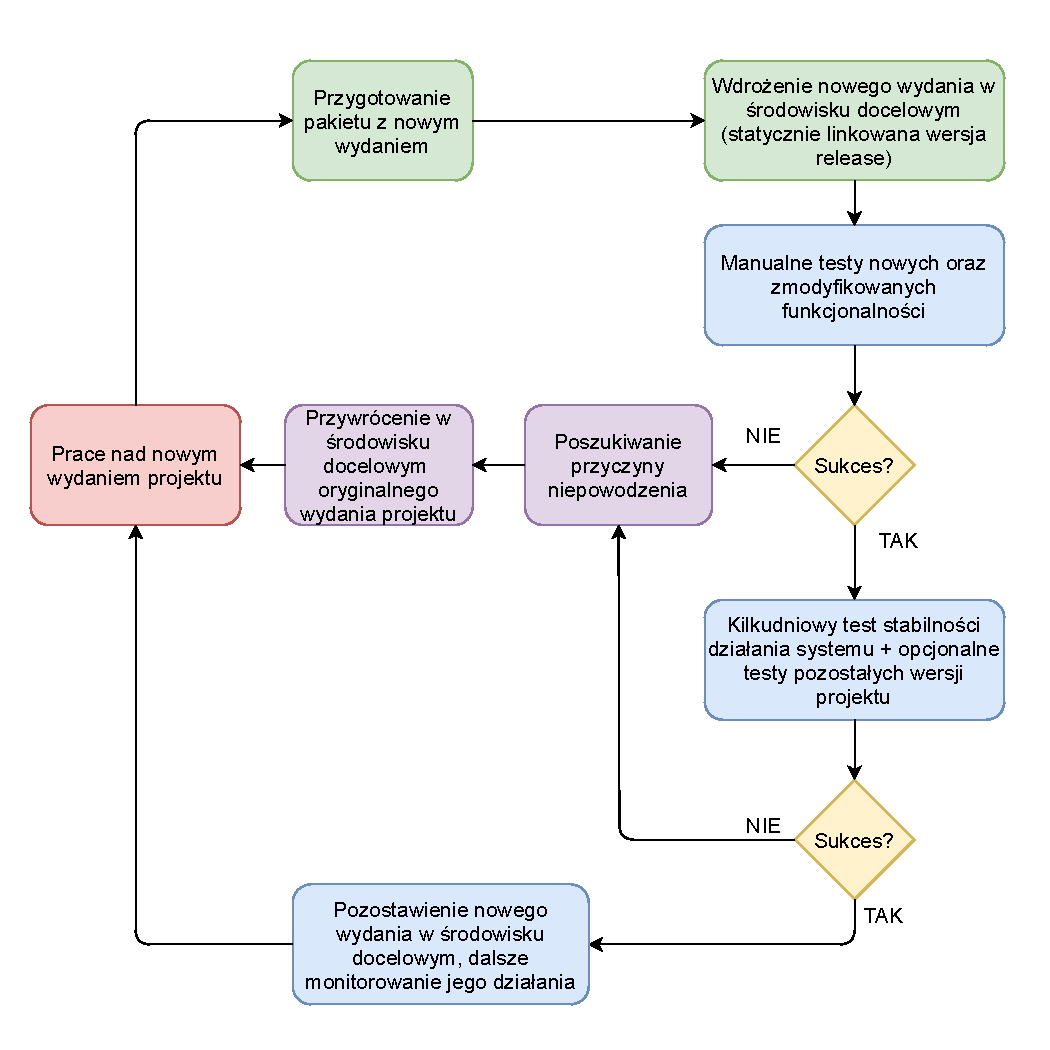
\includegraphics[width=0.85\textwidth]{algorithm.pdf}
\caption{Diagram przedstawiający stosowany przez autorów cykl pracy - kolorem niebieskim oznaczone zostały etapy związane z~regularnymi testami oprogramowania.}
\label{fig:tests_1}
\end{figure}

\section{Testy po migracji systemu (JC)}

Jednym z~ważniejszych etapów pracy magisterskiej była migracja całego systemu GGSS wraz ze sprzętem elektronicznym do nowego środowiska uruchomieniowego. Polegała ona na przeniesieniu kopii oprogramowania na nowy komputer oraz podłączeniu do niego wykorzystywanych urządzeń.

Cała operacja miała odbywać się w~ramach wyjazdu autorów do CERN, natomiast ze względów pandemicznych wyjazd ten został ostatecznie odwołany. Z~tego powodu migracja mogła zostać jedynie częściowo przeprowadzana przez autorów, znaczną część pracy wykonali natomiast eksperci, którzy znajdowali się na miejscu. W~ramach migracji podłączyli oni sprzęt oraz przenieśli zawartość dysków ze starego komputera do nowej maszyny. Przed uruchomieniem całego systemu autorzy zdalnie zweryfikowali poprawność całego procesu. W~ramach tego etapu wykorzystane zostały aplikacje do testowania sprzętu opisane w~sekcji \ref{ch:hardware_testing}. W~trakcie wykonywania testów sprzętu okazało się, że jedynie urządzenie połączone bezpośrednio do komputera jest wykrywane, a~urządzenia połączone za pomocą hub'u USB nie. Rozwiązaniem problemu było podłączenie dodatkowego zasilania wymaganego przez wcześniej wspomniany hub. Upewniwszy się iż sprzęt podłączony jest poprawnie i~jego działanie nie budzi zastrzeżeń, autorzy wykonali sprawdzenia pozostałych elementów środowiska, czyli: zainstalowanych bibliotek, wpisów w~tabeli programu \lstinline{crontab} oraz poprawności umieszczenia plików projektu.

Po sprawdzeniu wszystkich wymaganych elementów środowiska autorzy rozpoczęli proces uruchamiania projektu GGSS wraz z~jego główną aplikacją. W~jego trakcie dokładnie monitorowano zachowanie warstwy oprogramowania oraz urządzeń elektronicznych. Oprócz zachowania aplikacji sprawdzane było również zużycie zasobów oraz ewentualne błędy, które mogły wystąpić ze względu na migrację. Po uruchomieniu projektu monitorowano jego działanie przez kilka godzin, a~następnego dnia dokonano sprawdzenia dziennika zdarzeń. Nie stwierdzono żadnych problemów z~systemem, a~całość działała poprawnie. Migracja została uznana za zakończoną z~sukcesem.

\section{Testy wersji finalnej (AK i~JC)}
Niniejsza sekcja stanowi opis testów finalnej wersji systemu GGSS wykonanych w~sierpniu 2021 roku. Sprawdzeniu poddane zostały zarówno wszystkie najważniejsze funkcjonalności systemu, jak również elementy infrastruktury projektu oraz wprowadzone przez autorów zmiany. Ponadto zbadane zostało zużycie zasobów systemu, takich jak pamięć, podczas długotrwałego, nieprzerwanego działania aplikacji \emph{ggss-runner}. 

\subsection{Testy funkcjonalności głównej aplikacji}
Autorzy dokonali szczegółowego sprawdzenia wszystkich przygotowanych modyfikacji i~rozszerzeń. Ponadto testowane były elementy wchodzące w~skład projektu od początku jego działania. W~kolejnych akapitach opisane zostały poszczególne scenariusze testowe wraz z~otrzymanymi przez autorów wynikami.

\subsubsection*{Działanie komend dedykowanych zasilaczom wysokiego napięcia}
Testom poddana została przygotowana przez autorów składnia komend służących do komunikacji z~zasilaczami wysokiego napięcia. Wykonane zostały sprawdzenia wszystkich trzech typów poleceń (MON, SET, RAW) przy zastosowaniu zróżnicowanych konfiguracji opisujących moduły, kanały oraz parametry. Ze względu na powtarzalny charakter przeprowadzonych sprawdzeń, autorzy zdecydowali się jedynie na przytoczenie wybranych przykładów - wykonane testy obejmowały natomiast wszystkie wspierane parametry komend oraz obsługę wszystkich znanych błędów i~sytuacji wyjątkowych, takich jak niepoprawny format komendy czy typ przekazywanej wartości. Weryfikacja wykonywana była zarówno za pomocą paneli w~środowisku WinCC OA, jak również za pomocą dedykowanego skryptu \lstinline{dimhw.sh}. Listing \ref{lst:test_hw_1} przedstawia przykład testu komendy typu MON, pobierającej wartość oczekiwanego i~monitorowanego napięcia dla wszystkich kanałów każdego z~zasilaczy. Listing \ref{lst:test_hw_2} przedstawia natomiast weryfikację komendy typu SET, zmieniającej wartość napięcia na jednym z~kanałów na wartość 1. Listing \ref{lst:test_hw_3} zawiera przykład wykorzystania komendy typu RAW. Sprawdzenie obsługi sytuacji wyjątkowych zaprezentowane zostało na listingu \ref{lst:test_hw_4}, gdzie do systemu podawana jest niepoprawna nazwa (alias) zasilacza wysokiego napięcia. Testy zakończyły się powodzeniem - wszystkie sprawdzane scenariusze zwróciły wynik zgodny z~oczekiwaniami.

\lstinputlisting[
    language=Cmd, 
    caption={Przykład testu sprawdzającego działanie komendy typu MON, sprawdzającej wartości parametrów VSET i~VMON dla wszystkich kanałów każdego z~zasilaczy.}, 
    label={lst:test_hw_1}
]{6_tests/code_samples/dim_hw_mon.txt}

\lstinputlisting[
    language=Cmd, 
    caption={Przykład testu sprawdzającego działanie komendy typu SET, ustawiającej napięcie na jednym z~kanałów na wartość 1.}, 
    label={lst:test_hw_2}
]{6_tests/code_samples/dim_hw_set.txt}

\lstinputlisting[
    language=Cmd, 
    caption={Przykład testu sprawdzającego działanie komendy typu RAW, sprawdzającej wartość monitorowanego natężenia prądu (parametr IMON) na wybranym kanale.}, 
    label={lst:test_hw_3}
]{6_tests/code_samples/dim_hw_raw.txt}

\lstinputlisting[
    language=Cmd, 
    caption={Przykład testu sprawdzającego zachowanie systemu w~sytuacji, gdy przekazana została niepoprawna nazwa urządzenia.}, 
    label={lst:test_hw_4}
]{6_tests/code_samples/dim_hw_error.txt}

\subsubsection*{Opróżnianie bufora urządzenia MCA}
Sprawdzone zostało poprawne wykonanie algorytmu pozwalającego na zapobieganie przepełnieniu bufora urządzenia MCA poprzez cykliczne przenoszenie jego zawartości do pamięci RAM komputera. Weryfikacji poddane zostały zarówno scenariusze, w~których mechanizm ten nie jest stosowany (np. gdy wartość parametru \lstinline{mcaRefreshInterval} ustawiona została na 0) - wtedy oczekiwanym rezultatem było przepełnienie bufora, jak również te, gdy algorytm był wykorzystywany. Stosowanie przygotowanego rozszerzenia pozwoliło uniknąć błędu przepełnienia bufora, a~zatem umożliwiło pobranie większej ilości danych. Badane były ponadto przypadki specjalne, takie jak wybór większej niż czas pomiaru wartości parametru \lstinline{mcaRefreshInterval} (w tym przypadku system powinien wykonać pobranie danych jedynie przy aktualizacji ELMB w~połowie pomiaru oraz po zakończeniu zbierania danych). Wszystkie testy przyniosły oczekiwane rezultaty, a~zatem przygotowana funkcjonalność działa w~sposób poprawny.

\subsubsection*{Działanie komend sterujących systemem GGSS}
Autorzy poddali testom działanie wszystkich przygotowanych lub zmodyfikowanych komend sterujących systemem GGSS, takich jak: \lstinline{update}, \lstinline{update spectrum} czy też \lstinline{reset channelsOrder}. Ponieważ ich dokładne działanie przedstawione zostało w~części pracy poświęconej przygotowanym ulepszeniom, informacje te nie zostaną tu powtórzone. Podobnie jak w~przypadku pozostałych funkcjonalności, sprawdzane były również przypadki specjalne, takie jak wybór nieistniejącej konfiguracji parametrów początkowych przy dopasowywaniu krzywej do zebranych danych czy też próba przywrócenia oryginalnej kolejności liczników słomkowych, gdy system GGSS nie został zatrzymany. Wszystkie testy zakończyły się zgodne z~przewidywanym zachowaniem systemu. Ponadto sprawdzeniu poddane zostały niektóre z~komend istniejących w~systemie przed modyfikacjami - one również działają poprawnie.

\subsubsection*{Działanie algorytmu dopasowującego krzywą do zebranych danych}
Sprawdzone zostało działanie nowego algorytmu pozwalającego na wyznaczenie parametrów początkowych wykorzystywanych do przeprowadzania dopasowania krzywej do zebranych danych. W~tym przypadku wykonane zostały szczególnie kompleksowe testy, ponieważ przygotowany algorytm ma kluczowy, bezpośredni wpływ na działanie całego systemu. Sprawdzone zostały zatem różne wartości opisujące zakres, w~jakim poszukiwane ma być maksimum lokalne (tzw. \emph{fit range}) - zarówno obejmujące poszukiwany punkt (wtedy oczekiwano sukcesu), jak i~niezawierające go (w takim przypadku oczekiwanym wynikiem był błąd). Ponadto sprawdzone zostały różne wartości parametru \lstinline{smoothingWindowHalf}, odpowiedzialnego za jakość wygładzenia danych za pomocą stosowanego filtru. Szczególnym przypadkiem była tutaj wartość 0~oznaczająca, że algorytm nie powodował zmiany w~danych. Testom poddane zostały ponadto wszystkie cztery konfiguracje parametrów początkowych i~typów dopasowywanej funkcji: \lstinline{GaussFitXe}, \lstinline{GaussFitAr}, \lstinline{Gauss2FitXe} oraz \lstinline{Gauss2FitAr}. Ponadto działanie przygotowanych modyfikacji sprawdzone zostało w~sposób długoterminowy - poprzez monitorowanie poprawności działania systemu w~czasie przeprowadzania testów zużycia zasobów. Autorzy nie wykryli niedoskonałości w~przygotowanym rozwiązaniu, a~zatem uznane zostało ono za poprawne.

\subsubsection*{Pozostałe testy}
Wykonując opisane do tej pory sprawdzenia, autorzy przeprowadzali ponadto szereg testów weryfikujących działanie innych funkcjonalności, zarówno tych modyfikowanych przez nich w~czasie prac nad jakością kodu, jak i~tych niezmienionych. Weryfikacji poddane zostało zatem działanie operacji na plikach i~strukturze XML (odczyt, modyfikacja), tworzenie dziennika zdarzeń czy modyfikowanie kolejności, w~jakiej wykonywany jest pomiar na poszczególnych licznikach słomkowych. Sprawdzane były ponadto funkcjonalności takie jak zerowanie napięć na zasilaczach w~momencie, gdy system kończy swoje działanie. Ponadto, za pomocą istniejących w~ramach infrastruktury WinCC OA paneli przetestowana została możliwość modyfikacji każdego parametru systemu. Przykład panelu pozwalającego na przeprowadzenie tego typu testów przedstawiony został na rysunku \ref{fig:panel-params}. Autorzy dochodzą zatem do wniosku, że z~punktu widzenia oferowanych funkcjonalności system GGSS działa w~pełni poprawnie.

\clearpage
\begin{figure}[H]
    \centering
    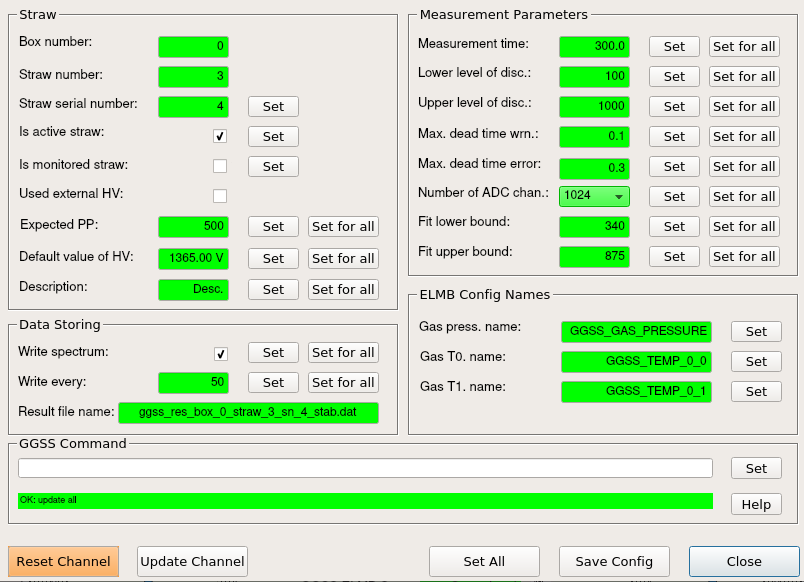
\includegraphics[width=\textwidth]{panel_params.png}
    \caption{Wykorzystany podczas testów panel pozwalający na monitorowanie i~modyfikację parametrów jednego licznika słomkowego.}
    \label{fig:panel-params}
\end{figure}


\subsection{Testy aplikacji oraz skryptów do obsługi urządzeń}

W~ramach testów wersji finalnej przeprowadzono sprawdzenie wszystkich aplikacji do obsługi sprzętu fizycznego, które były modyfikowane, czy też utworzone od zera przez autorów. Testy były przeprowadzane w~środowisku produkcyjnym przy wyłączonym systemie GGSS, a~dokładnie z~wyłączoną główną aplikacją projektu. W~celu sprawdzenia poprawności działania oraz funkcjonalności wykonano zarówno komendy z~użyciem trybu interaktywnego utworzonych aplikacji, jak i~trybu scenariuszowego. W~pierwszej kolejności testom została poddana aplikacja odpowiedzialna za obsługę zasilacza wysokiego napięcia, czyli \emph{high-voltage-service-app}. Listing \ref{lst:high-voltage-service-app-startup} przedstawia wywołanie aplikacji z~wszystkimi wymaganymi argumentami oraz jej wiadomość powitalną. W~ramach tejże wiadomości prezentowane są informację o~utworzeniu połączenia z~modułem zasilacza. Następnie wyświetlana jest informacja o~wykorzystaniu trybu interaktywnego wraz z~krótką pomocą zawierającą format komend.

\clearpage
\lstinputlisting[
    language=Cmd,
    caption={Uruchomienie aplikacji \emph{high-voltage-service-app} w~trybie interaktywnym.},
    label={lst:high-voltage-service-app-startup}
]{6_tests/code_samples/high-voltage-service-app-startup.txt}

Listing \ref{lst:high-voltage-service-app-commands} zawiera przykład działania komend pozwalających na ustawienie wartości napięcia na wyjściu zasilacza, oraz pobrania tejże wartości wraz z~asercją mającą na celu automatyczne sprawdzenie, czy oczekiwana wartość jest zgodna z~rzeczywistą. Trzecie wywołanie komendy ma za zadania sprawdzenie, czy w~przypadku nieotrzymania zadanej wartości aplikacja poprawnie zgłosi błąd. Ostatnie z~wywołań sprawdza poprawność działania asercji z~tolerancją.

\lstinputlisting[
    language=Cmd,
    caption={Komendy wykonywane w~trybie interaktywnym aplikacji \emph{high-voltage-service-app}.},
    label={lst:high-voltage-service-app-commands}
]{6_tests/code_samples/high-voltage-service-app-commands.txt}

Testom poddany został również tryb scenariuszowy, co przedstawia listing \ref{lst:high-voltage-service-app-scenario}. W~tym przypadku najpierw wyświetlane są informacje o~komendach przetworzonych w~ramach danego pliku scenariuszowego, a~dopiero później następuje ich uruchomienie, zgodnie ze specyfikacją zawartą w~argumentach wywołania aplikacji.

\lstinputlisting[
    language=Cmd,
    caption={Przykładowe uruchomienie aplikacji \emph{high-voltage-service-app} w~trybie scenariuszowym. Zawartość scenariusza została skrócona na potrzeby manuskryptu.},
    label={lst:high-voltage-service-app-scenario}
]{6_tests/code_samples/high-voltage-service-app-scenario.txt}

Wszystkie testy aplikacji \emph{high-voltage-service-app} przebiegły pomyślne. Aplikacja wykonała wszystkie żądane czynności, a~odpowiednie wartości pojawiły się na zasilaczu wysokiego napięcia. Zarówno tryb interaktywny, jak i~scenariuszowy zostały uruchomione bez problemu. Aplikacja zachowywała się poprawnie również w~przypadku, gdy oczekiwane było zgłoszenie błędu.

Następnie w~podobny sposób przetestowane zostało dzianie aplikacji \emph{multiplexer-service-app}. Przetestowano zarówno jej tryb interaktywny, jak i~scenariuszowy. Ze względu na to, że testy wyglądały analogicznie jak w~przypadku aplikacji \emph{high-voltage-service-app}, a~różnice stanowiły jedynie komendy oraz odpowiedzi od urządzenia, zaprezentowany został jedynie listing \ref{lst:multiplexer-service-app}, który przedstawia wiadomość powitalną aplikacji do obsługi multipleksera oraz kilka podstawowych komend.

\clearpage
\lstinputlisting[
    language=Cmd,
    caption={Przykład działania aplikacji \emph{multiplexer-service-app} - przedstawiona została wiadomość powitalna zawierająca informacje na temat możliwości aplikacji oraz wykonanie kilku przykładowych komend, powodujących pobranie numeru seryjnego urządzenia oraz pobranie i~zmianę aktywnego kanału.},
    label={lst:multiplexer-service-app}
]{6_tests/code_samples/multiplexer-service-app.txt}

W~przypadku aplikacji \emph{multiplexer-service-app} wszystkie testy udało się przeprowadzić pomyślnie. Nie stwierdzono żadnych błędów w~działaniu wyżej wymienionej aplikacji. Wszystkie funkcjonalności, tryb interaktywny, jak i~tryb scenariuszowy działały poprawnie.

\clearpage
Testy aplikacji \emph{high-voltage-killer} oraz skryptów składających się na system awaryjnego wyłączania wysokiego napięcia polegały zarówno na uruchomieniu samego programu i~sprawdzeniu, czy jego działanie jest poprawne oraz na symulowaniu rzeczywistych warunków, w~ramach których program powinien zostać uruchomiony. 

W~pierwszej kolejności wykorzystano wcześniej przetestowaną aplikację \emph{high-voltage-service-app} w~celu ustawienia napięcia na zasilaczu wysokiego napięcia na wartość większą niż zero, następnie uruchomiono aplikację \emph{high-voltage-killer}, co przedstawia listing \ref{lst:high-voltage-killer}. W~ramach działania aplikacja analizuje znajdujące się w~systemie pliki urządzeń, następnie wybiera te, za pomocą których podłączone są zasilacze wysokiego napięcia. Następnie, wykorzystując bibliotekę \emph{caenn1470-lib}, zerowane są napięcia na wszystkich wyjściach wszystkich podłączonych modułów. Aplikacja prewencyjne próbuje zerować napięcia na modułach od 0~do 7, nawet, gdy tylko 3~moduły są uruchomione, natomiast komendy wysyłane są jedynie do podłączonych modułów.

\lstinputlisting[
    language=Cmd,
    caption={Uruchomienie aplikacji \emph{high-voltage-killer}},
    label={lst:high-voltage-killer}
]{6_tests/code_samples/high-voltage-killer.txt}

Następnie ponownie wykorzystując aplikację \emph{high-voltage-service-app} sprawdzono, czy rzeczywiście napięcie zostało wyzerowane. Wykonując odpowiednie komendy stwierdzono, że test przebiegł pomyślnie. Oprócz samego działania aplikacji \emph{high-voltage-killer} przetestowano również funkcjonalności dostarczane w~skryptach współpracujących z~tą aplikacją:
\begin{itemize}
    \item Uruchomienie aplikacji \emph{high-voltage-killer} jeżeli główna aplikacja GGSS przestała działać i~nie została uruchomiona w~przeciągu 5~minut
    \item Możliwość zablokowania systemu awaryjnego wyłączania zasilania poprzez utworzenie pliku blokady.
    \item Ciągłe działanie systemu awaryjnego wyłączania zasilania w~przypadku braku pliku blokady.
    \item Awaryjne wyłączenie zasilania w~przypadku otrzymania sygnału SIGTERM
\end{itemize}

Przeprowadzone testy wszystkich wyżej wymienionych funkcjonalności przebiegły pomyślnie. Nie napotkano żadnych przeszkód w~trakcie ich wykonywania. Dodatkowo przeprowadzono testy aplikacji \emph{device-detector}, której zadaniem jest raportowanie informacji o~podłączonych do systemu urządzeniach, które wymagane są do działania systemu GGSS. Również w~tym przypadku proces przebiegł pomyślne. W~celu osiągnięcia pewności, iż wszystkie aplikacje związane ze sprzętem fizycznym działają poprawnie w~nowym środowisku testom została poddana również aplikacja \emph{mca-service-app}. Uruchomienie tejże aplikacji nie spowodowało żadnych problemów, a~wyniki jej działania były poprawne. Wraz z~zakończeniem tego testu wszystkie aplikacje oraz skrypty związane ze sprzętem zostały w~pełni przetestowane, dzięki czemu autorzy mogli być pewni poprawności zaimplementowanych funkcjonalności.


\subsection{Testy wykorzystania pamięci operacyjnej}

Zwieńczeniem testów, które miało zapewnić długotrwałe, bezproblemowe działanie projektu GGSS, było monitorowanie, przez długi okres czasu, zasobów systemowych przypisanych do głównej aplikacji. W~tym celu wykorzystano wcześniej opisany skrypt \lstinline{check_resource_usage_ggss.sh}. Najważniejszym monitorowanym parametrem był RSS (\emph{Resident Set Size}), który przedstawiał ilość pamięci RAM wykorzystywanej przez proces. Ze względu na to, że aplikacja \emph{ggss-runner} powinna działać bez zakłóceń przez okres co najmniej kilku miesięcy ważne było, aby test wykazał brak zwiększającego się zużycia pamięci, mogącego w~dłuższym okresie czasu doprowadzić do wyczerpania jej zasobów w~systemie.

Rysunek \ref{fig:rss-short} przedstawia ilość wykorzystywanej pamięci (RSS) względem czasu. Na rysunku przedstawiony został okres od dnia 10 sierpnia 2021 roku w~południe do końca dnia 11 sierpnia 2021 roku. W~trakcie tego okresu autorzy przeprowadzali testy z~wykorzystaniem platformy Valgrind, co widoczne jest na wykresie w~okresach, w~których zużycie pamięci znacząco odstaje od normy, która plasuje się w~okolicach 6000 kB. Dnia 10 sierpnia 2021 roku autorzy wykonywali testy z~wykorzystaniem narzędzia Massif - w~trakcie korzystania z~tego narzędzia zużycie pamięci wynosiło niecałe 50 tysięcy kB. W~przypadku odstępstwa z~dnia 11 sierpnia wykorzystane zostało narzędzie Memcheck, a~zużycie pamięci wyniosło znacznie powyżej 200 tysięcy kB. Na wykresie widoczny jest również charakterystyczny ogon związany z~ponownym uruchomieniem aplikacji. Wynika on z~faktu, iż aplikacja w~fazie inicjalizacji oraz w~trakcie początkowych pomiarów alokuje pamięć na wszystkie potrzebne zmienne wraz z~buforami na przechowywanie danych pozyskanych z~urządzeń fizycznych wchodzących w~skład systemu GGSS.

\clearpage
\begin{figure}[H]
    \centering
    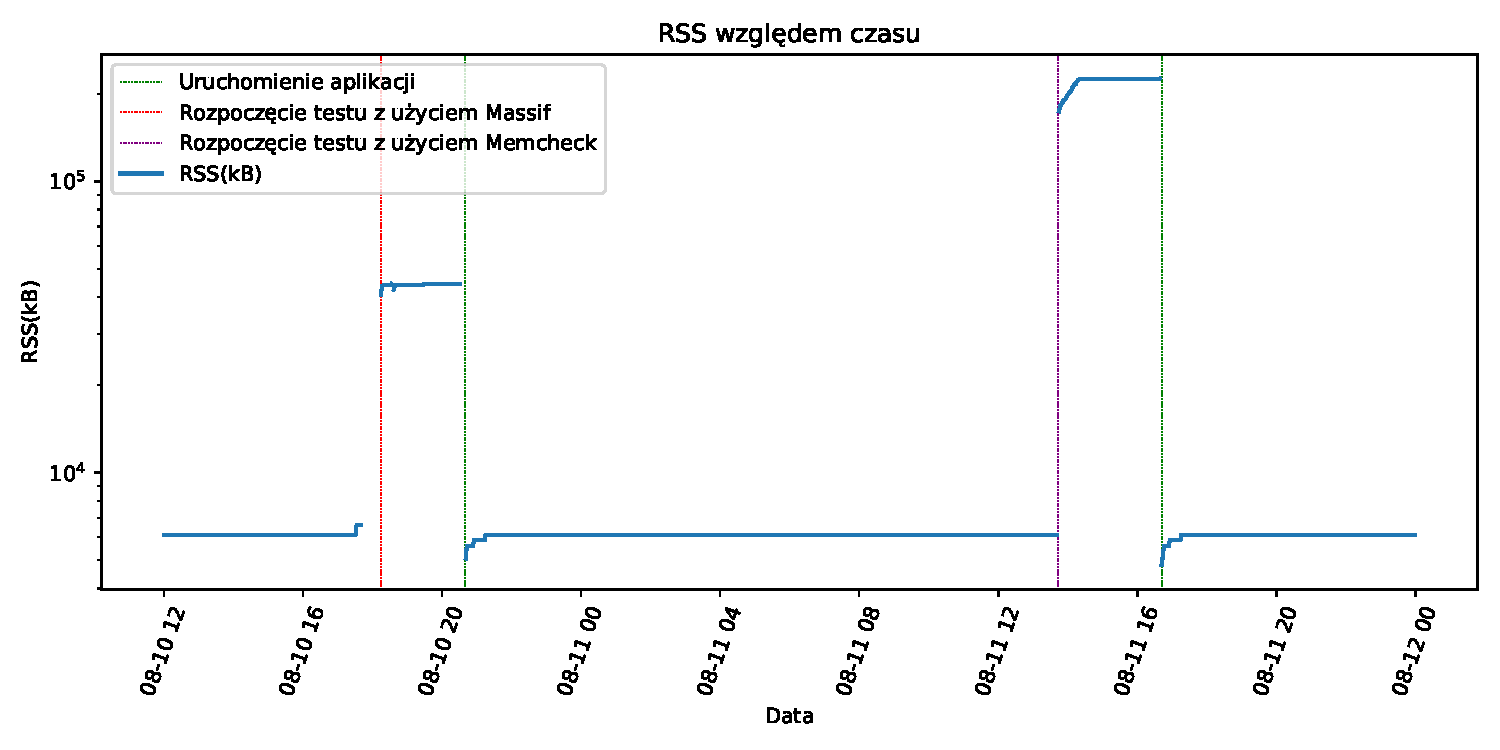
\includegraphics[width=0.9\textwidth]{rss_short.pdf}
    \caption{Wykres przedstawiający zużycie pamięci (RSS) przez aplikację \emph{ggss-runner} względem czasu w~okresie od 10 sierpnia 2021 roku do końca 11 sierpnia 2021 roku.}
    \label{fig:rss-short}
\end{figure}

W~celu dokładniejszej weryfikacji długotrwałego zużycia pamięci przygotowany został również rysunek \ref{fig:rss-long}. Przedstawia on parametr RSS względem czasu dla dłuższego okresu monitorowania. Oprócz charakterystycznych odstępstw od normy związanych z~wykorzystaniem platformy Valgrind nie zaobserwowano żadnych anomalii. Zmiany ilości wykorzystywanej pamięci wiązały się jedynie z~początkową inicjalizacją zmiennych, buforów na dane, czy też wynikały z~interakcji z~systemem, np.: poprzez wysłanie do niego komend. W~przypadku, gdy aplikacja \emph{ggss-runner} działała bez zewnętrznych poleceń, czy też zakłóceń, to zużycie pamięci nie zwiększało się przez dłuższy okres czasu.

\begin{figure}[H]
    \centering
    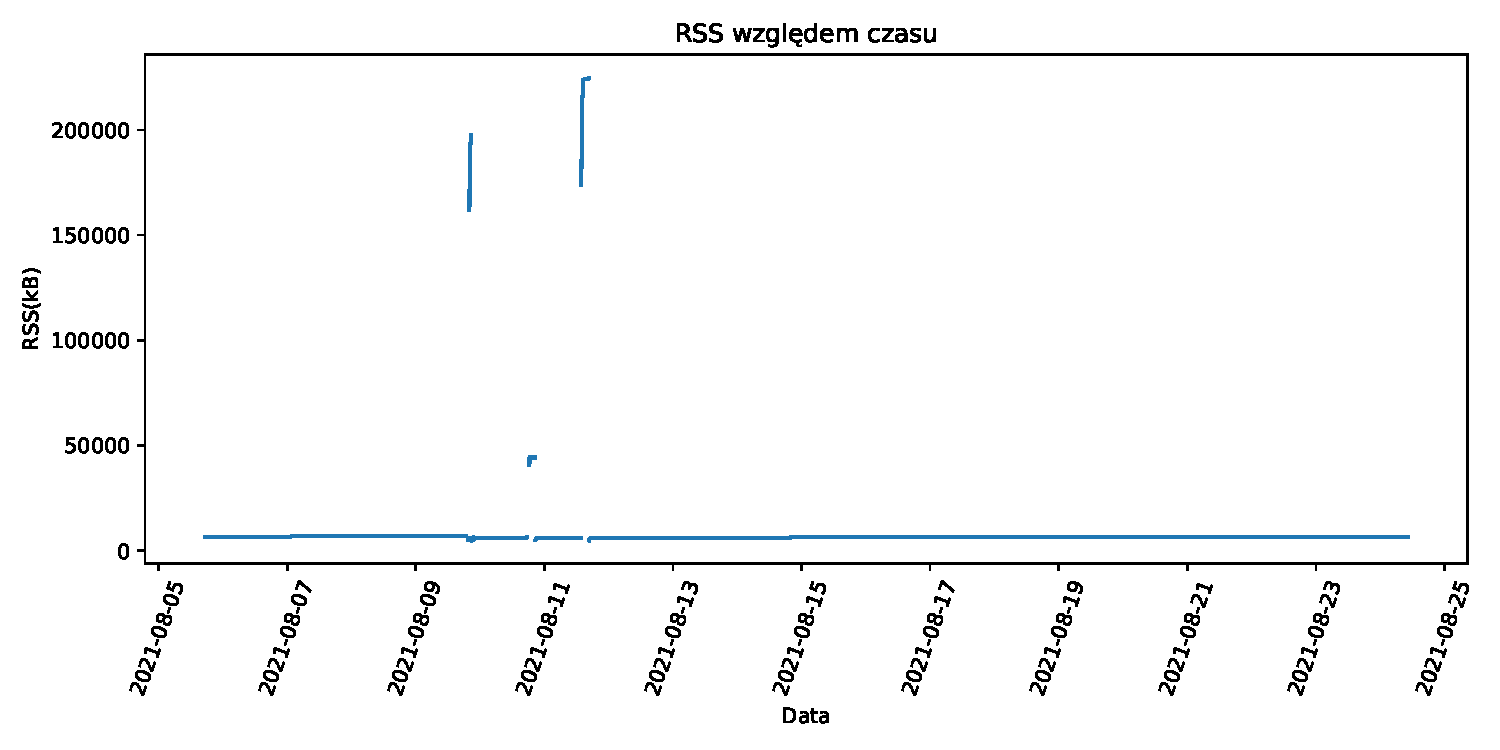
\includegraphics[width=0.9\textwidth]{rss_long.pdf}
    \caption{Wykres przedstawiający zużycie pamięci (RSS) przez aplikację \emph{ggss-runner} względem czasu w~okresie od 5~sierpnia 2021 roku do 25 sierpnia 2021 roku.}
    \label{fig:rss-long}
\end{figure}

W~celu zbadania występowania potencjalnych błędów w~zarządzaniu wykorzystania pamięcią użyto narzędzie Memcheck wchodzące w~skład platformy Valgrind. Testy wykazały obecność nieprawidłowości, jednakże wygenerowany raport wskazuje, że pochodzą one z~bibliotek zewnętrznych wykorzystywanych w~projekcie, w~tym przede wszystkim z~biblioteki DIM oraz Boost.Log. Na listingu \ref{lst:memcheck-error} umieszczony został fragment raportu z~działania narzędzia Memcheck prezentujący przykładowy błąd związany z~faktem, że biblioteka DIM nie dokonuje poprawnego zwolnienia alokowanej pamięci. Po analizie wszystkich zgłoszonych przez narzędzie błędów, autorzy stwierdzili, że żaden z~nich nie powoduje stopniowego wzrostu wykorzystywanej pamięci operacyjnej. Na tej podstawie zostało stwierdzone, że nie zagrażają one bezpieczeństwu długotrwałego działania aplikacji.

\lstinputlisting[
    language=Cmd,
    caption={Przykładowy, powodowany przez bibliotekę DIM, błąd raportowany przez narzędzie Memcheck.},
    label={lst:memcheck-error}
]{6_tests/code_samples/memcheck-error.txt}

Dodatkowym argumentem przemawiającym za poprawnością wyżej przytoczonych wniosków jest fakt, iż niezależnie od długości przeprowadzanego testu z~użyciem narzędzia Memcheck rozmiar pamięci oznaczonej jako \lstinline{still reachable} pozostawał niezmienny i~wynosił ok 178kB, co zostało zaprezentowane na listingu \ref{lst:memcheck-leak-summary}.

\lstinputlisting[
    language=Cmd,
    caption={Podsumowanie wycieków pamięci raportowane przez narzędzie Memcheck.},
    label={lst:memcheck-leak-summary}
]{6_tests/code_samples/memcheck-leak-summary.txt}

Przeprowadzone zostały również, trwające nieco poniżej dwóch godzin, testy zużycia pamięci sterty i~stosu z~wykorzystaniem narzędzia Massif wchodzącym w~skład platformy Valgrind. Wynik zaprezentowany został na rysunku \ref{fig:massif-long}. W~początkowym etapie testu widoczne jest stopniowe wzrastanie zużycia pamięci. Wynika ono z~przeprowadzania pierwszych iteracji pomiarów na wszystkich licznikach słomkowych podczas których alokowana jest pamięć pozwalająca na przechowywanie wyników z~ostatnich kilku iteracji dla danego licznika. Następnie zużycie pamięci pozostaje stałe, aż do momentu rozpoczęcia procesu zakańczania działania programu, gdy rośnie ono na krótką chwilę. Przeprowadzony test dowodzi, że w~czasie regularnego działania systemu zużycie pamięci pozostaje stałe.

\begin{figure}[H]
    \centering
    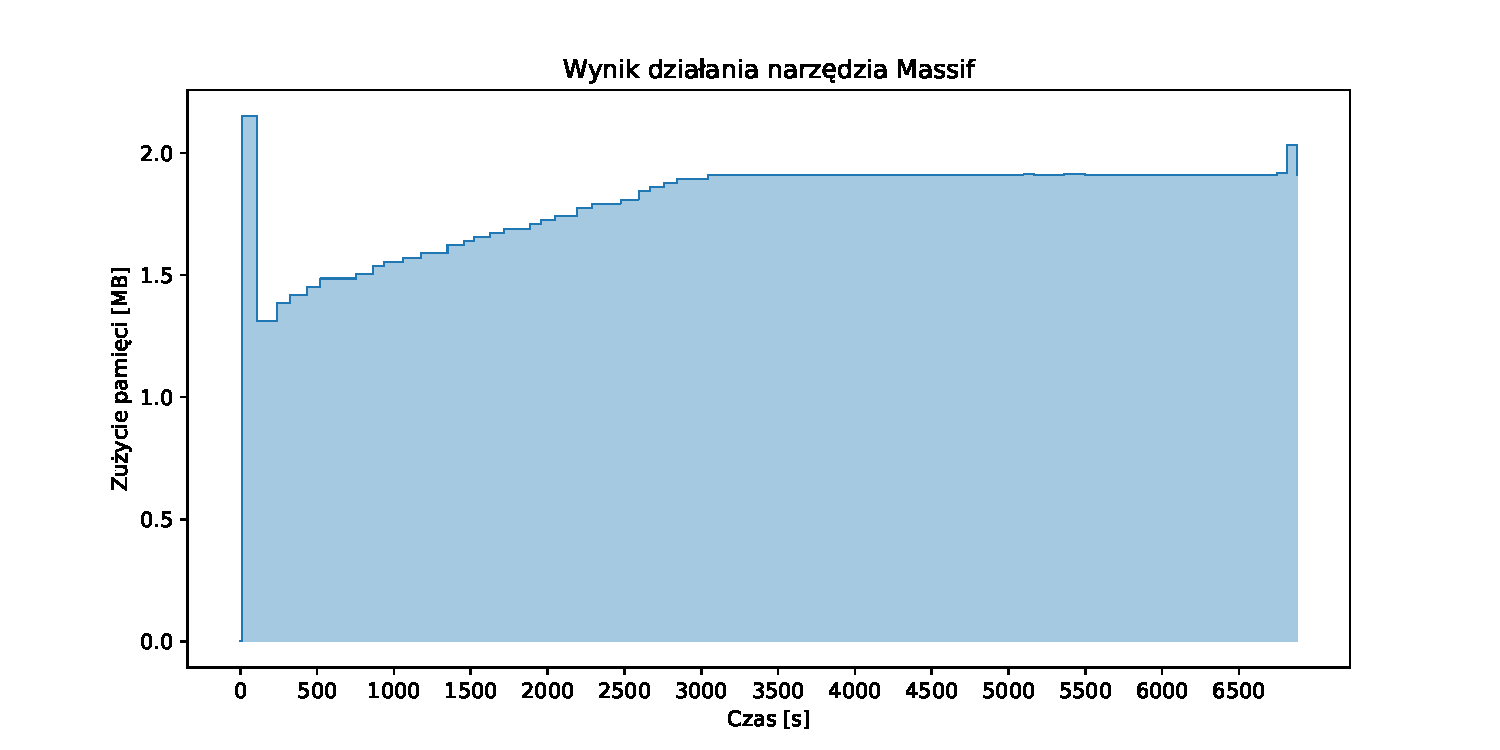
\includegraphics[width=\textwidth]{massif_plot_long.pdf}
    \caption{Wykres przedstawiający zużycie pamięci sterty i~stosu zbadane z~wykorzystaniem narzędzia Massif.}
    \label{fig:massif-long}
\end{figure}

Przeprowadzone przez autorów testy wskazują na stabilne zachowanie programu pod kątem zużywanych zasobów systemowych, m.in. pamięci operacyjnej. Przeprowadzone zostały ponadto testy wykorzystania czasu procesora, które również wskazują na stabilne działanie programu.

\chapter{Podsumowanie (AK i JC)}
\label{cha:summary}

W niniejszym manuskrypcie zaprezentowane zostały wykonane przez autorów prace nad rozbudową i uaktualnieniem warstwy oprogramowania Systemu Stabilizacji Wzmocnienia Gazowego detektora ATLAS TRT. Zaprezentowane w kolejnych rozdziałach zmiany obejmowały szereg zróżnicowanych zagadnień, związanych zarówno z infrastrukturą projektu, jak i jego kodem źródłowym. 

Podczas wykonywania zaprezentowanych zadań autorzy zapoznali się z kodem źródłowym projektu. W pierwszych etapach prac wykonywano przede wszystkim niewielkie poprawki, których celem było poznanie systemu. Następnie autorzy rozszerzyli projekt o nowe funkcjonalności. Wszystkie założenia dotyczące wprowadzanych do systemu modyfikacji zostały spełnione, a każda wymagana funkcjonalność została zaimplementowana. Z punktu widzenia współczesnych praktyk programistycznych nie wszystkie zaproponowane rozwiązania są optymalne, jednakże wynika to przede wszystkim z nakładanych przez środowisko, w jakim działa projekt, ograniczeń.

W celu skutecznej organizacji projektu autorzy wykorzystali swoje doświadczenie pozyskane podczas prac nad komercyjnymi projektami informatycznymi. Stąd też duży nacisk położony został na odpowiednią organizację pracy oraz zastosowanie znanych praktyk ułatwiających pracę nad złożonymi systemami informatycznymi. Autorzy dokonali w nich oczywiście odpowiednich modyfikacji, by dostosować je do mniejszej skali projektu.

Podczas prac nad systemem autorzy starali się dołożyć wszelkich starań, by zapewnić jego niezawodność. O skuteczności tych działań świadczą przeprowadzone przez nich testy, jednoznacznie wskazujące na poprawność działania projektu. Szczególnie pomocne w zachowaniu odpowiedniej jakości okazały się regularne testy w środowisku docelowym, stosowanie testów automatycznych oraz rozbudowana infrastruktura automatyzująca czynności związane z cyklem życia oprogramowania.

Projekt pozostawiony został przez autorów w stanie umożliwiającym jego łatwy rozwój i utrzymanie. Aby dodatkowo ułatwić to zadanie, przygotowany został szereg instrukcji i poradników opisujących, w jaki sposób wykonywać zarówno podstawowe, jak i bardziej złożone działania. Praca nad systemem GGSS pozwoliła autorom na zdobycie cennego doświadczenia, zarówno z uwagi na prowadzoną pracę zespołową, jak i międzynarodowy charakter projektu. 



\printbibliography

\end{document}